\documentclass{article}

\usepackage{graphicx}
\usepackage{booktabs}
\author{Jan Ruman}
\date{30.8.2021}
\title{Analysis of activations in neural networks}

\begin{document}

\maketitle
\author
\date

\begin{abstract}
    In this work, we attempt to analyze the properties of activations inside
    of a neural network. Embeddings of activations inside trained and
    untrained neural network are compared across different layers.
    According to our results, activations from the trained network
    systematically outperform activations from the untrained network
    in terms of embedding quality.
\end{abstract}

\section{Introduction}
A neural network applies a sequence of non-linear transformations to its
input in order to produce an output. This procedure can be (and is)
done for all examples in the dataset. By storing the intermediate
transformations, we end up with multiple different representations of the
original dataset (possibly compressed and/or missing some information).

This work aims to analyze these representations in terms of their structure.
We are primarily interested in the way examples with the same class are
distributed when using the new representations.

\section{Methodology}
We will compare the data representations across two dimensions:
1) the depth of layer from which the representations were acquired and
2) whether the network was or was not trained. This means we will need
a neural network to be trained and datasets to train it on.

The representations are going to have many dimensions - it will be more
practical to use dimensionality reduction techniques that retain the
structure of the data. For that purpose, we are going to use t-SNE and UMAP
algorithms.

We need some way of comparing the structure of different representations.
Plotting embeddings acquired using dimensionality reduction techniques is
one of them, but some more rigorous approaches will be necessary to acquire
more reliable results. In order to measure the quality of a representation,
i.e., how well it clusters the same examples together and keeps different
examples away, we introduce several metrics in the next section.

A convolutional neural network with ReLU activation function will be used.
The first layer of the network is a convolutional layer and it consists of
4 filters of size 5. The second layer is a subsampling layer with kernel
size 2. The third layer is convolutional with 16 filters of size 3. The
fourth layer is subsampling layer with kernel size 2. The fifth layer
is convolutional with 64 filters of size 5. The sixth layer is fully
connected. ReLU activation function is applied after second, fourth, fifth
and sixth layer.

As representations, we will use:
\begin{itemize}
    \item the original dataset
    \item feature maps of the first layer (one for each filter)
    \item feature maps of the second layer (one for each filter)
    \item activations in the third layer (consisting of 64 1x1 feature maps)
\end{itemize}

We will use MNIST and FashionMNIST datasets. Because of memory limitations,
we will only work with a subset of 5 000 examples of each dataset.

\section{Embedding quality}
To measure the quality of a representation, we introduce several metrics that
capture the representation's properties. These properties then indicate how
good the representation is.

All except the last metric have distance as a unit. This is potentially
problematic as the absolute distance between points tells us nothing if we
do not know the distances between other points. It is thus necessary
to divide each of these metrics by the average distance between two points;
this will ensure that even though two embeddings have different scales, we
can still compare their metrics.

\subsection{Distances between points}
The first two metrics are concerned with an average distance between two points.
An average distance between points of the same class (\(d_s\)) and an average
distance between points of different classes (\(d_d\)) are measured. It is
quite obvious which one we would like to minimize and which one to maximize.

\subsection{Cluster centroids}
We can look at points belonging to the same class as a cluster. We introduce
two metrics using centroids of these clusters: 1) the total distance from 
points of a class to its centroid (\(c_s\)) and 2) the total distance between
different centroids (\(c_d\)).

\subsection{k-nearest neighbors}
We can use the k-nearest neighbors algorithm on the embedding to classify
examples in the dataset. The accuracy of k-nn (\(acc_{knn}\)) should
correlate with the quality of the embedding.

\section{Results}
Results presented in this part were acquired by running the
\texttt{\\ scripts/activations\_cnn.py} script. Output of this script
used in this document is part of the repository (in particular, the output
is stored in the \texttt{\\ out/activations\_cnn/} directory); rerunning
the script might give slightly different results.

In this work we will present only fraction of the visualizations actually
computed because of lack of space. The reader might see the rest of the
visualizations in the output directory mentioned above.

\subsection{MNIST}
First, we will look at embeddings produced by t-SNE. As there are 22
embeddings in total, it wouldn't be practical to show them all. Instead,
we are going to show one embedding per layer of the neural network. These
can be seen in Figures 1 to 7.

\begin{figure}
  \centering
    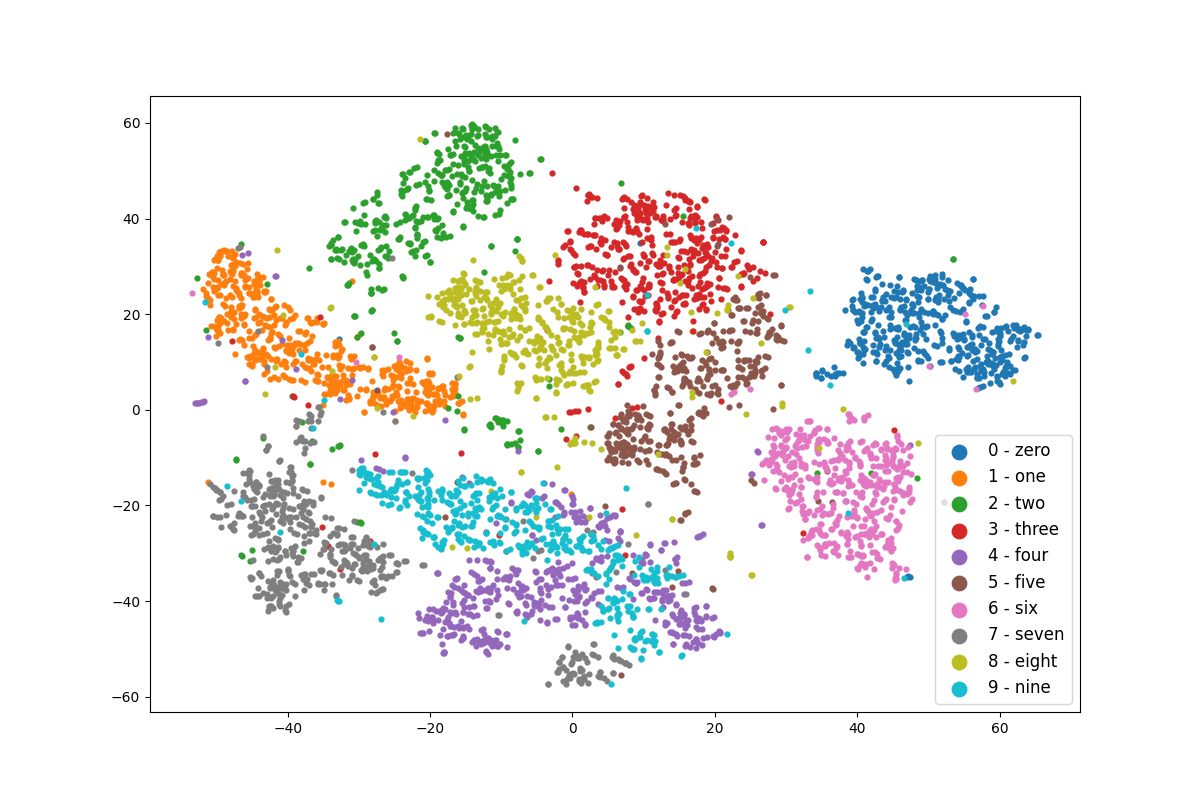
\includegraphics[width=1.0\textwidth]{../../out/activations_cnn/mnist/t-sne/trained/plot_l0.png}
    \caption{Embeddings of the original dataset (t-SNE).}
\end{figure}

\begin{figure}
  \centering
    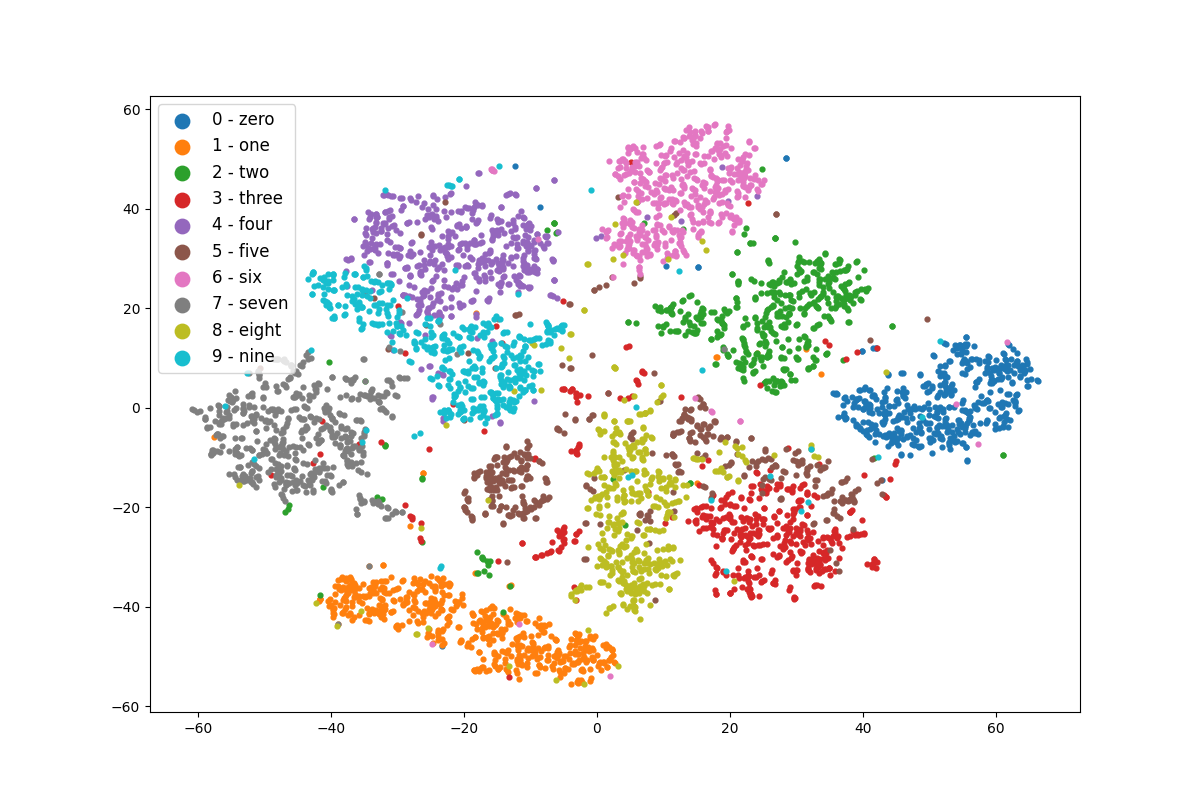
\includegraphics[width=1.0\textwidth]{../../out/activations_cnn/mnist/t-sne/trained/plot_l1_f0.png}
    \caption{Embeddings of activations in the first layer of a neural network trained on MNIST (t-SNE).}
\end{figure}

\begin{figure}
  \centering
    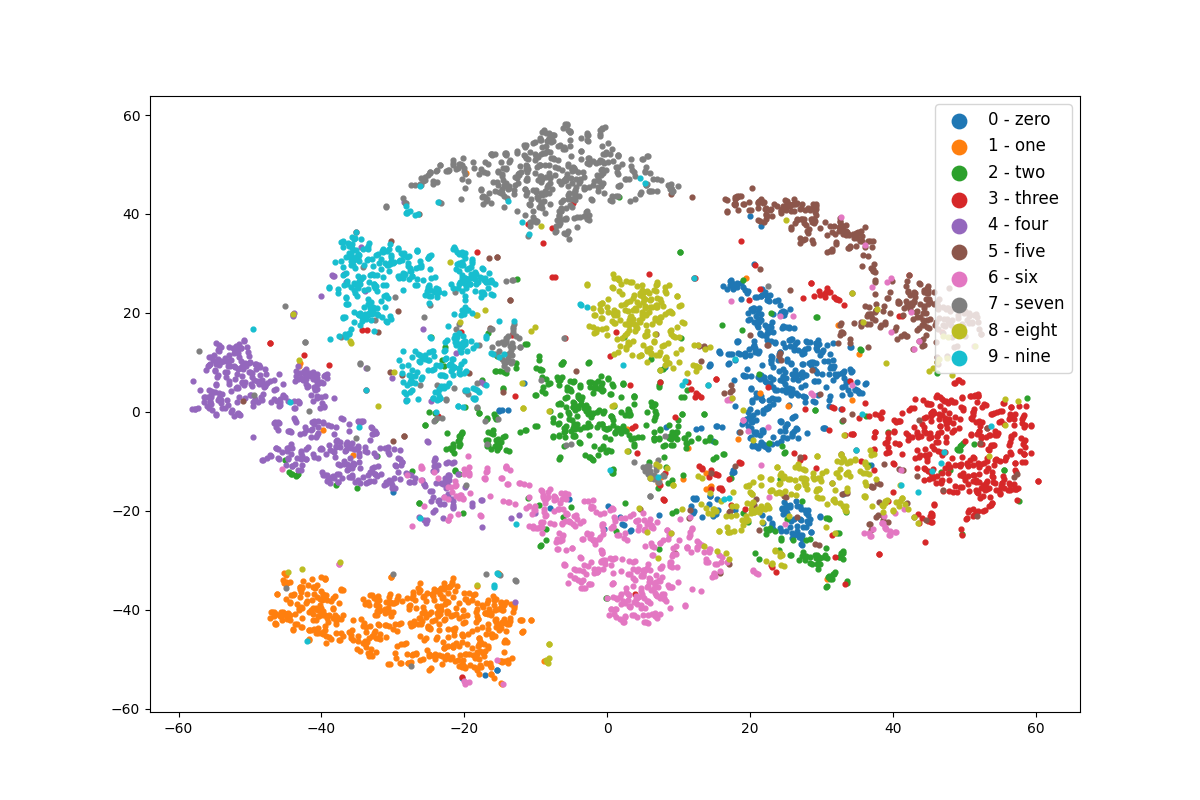
\includegraphics[width=1.0\textwidth]{../../out/activations_cnn/mnist/t-sne/trained/plot_l2_f0.png}
    \caption{Embeddings of activations in the second layer of a neural network trained on MNIST (t-SNE).}
\end{figure}

\begin{figure}
  \centering
    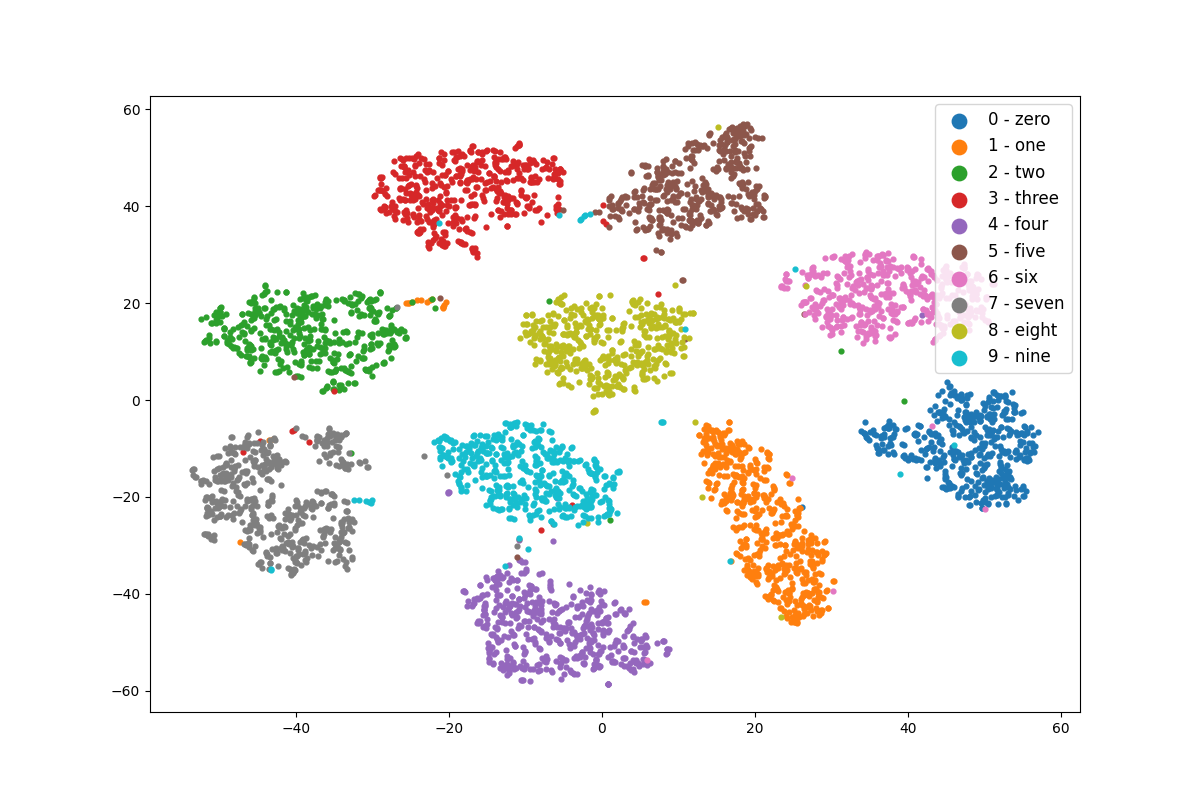
\includegraphics[width=1.0\textwidth]{../../out/activations_cnn/mnist/t-sne/trained/plot_l3.png}
    \caption{Embeddings of activations in the third layer of a neural network trained on MNIST (t-SNE).}
\end{figure}

\begin{figure}
  \centering
    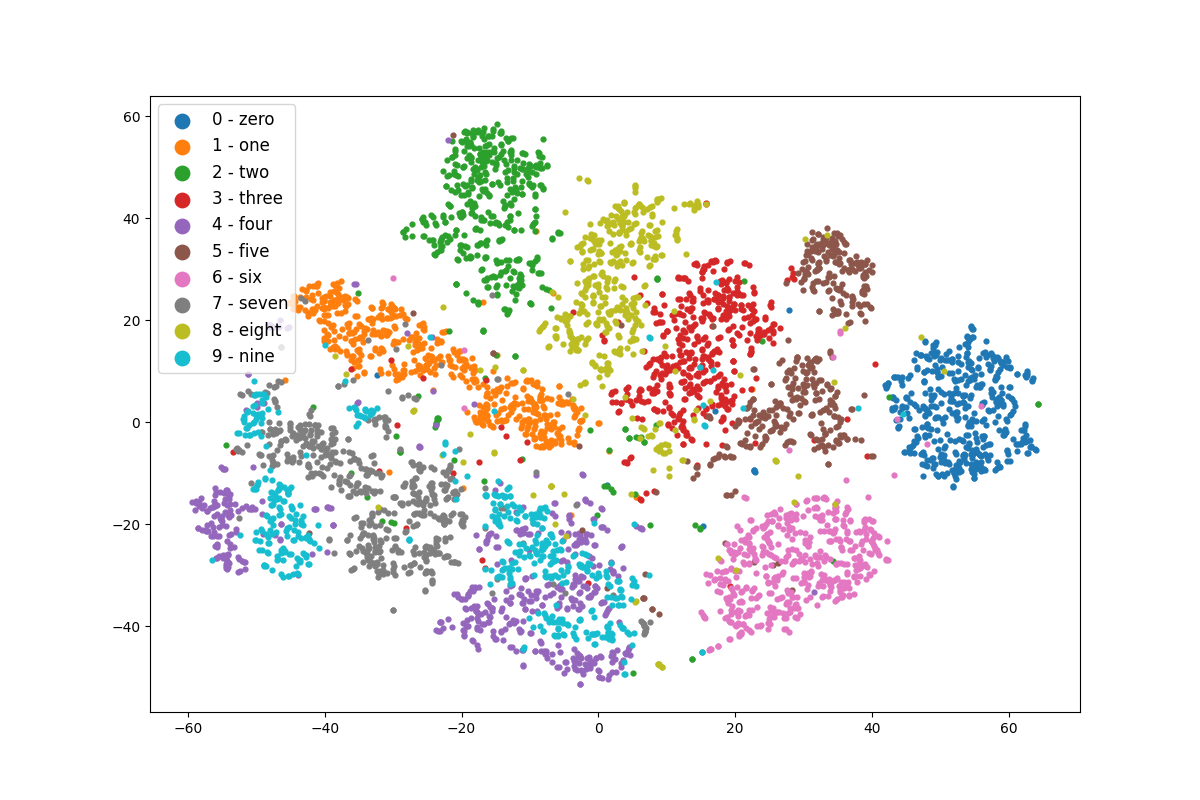
\includegraphics[width=1.0\textwidth]{../../out/activations_cnn/mnist/t-sne/untrained/plot_l1_f0.png}
    \caption{Embeddings of activations in the first layer of an untrained neural network (t-SNE).}
\end{figure}

\begin{figure}
  \centering
    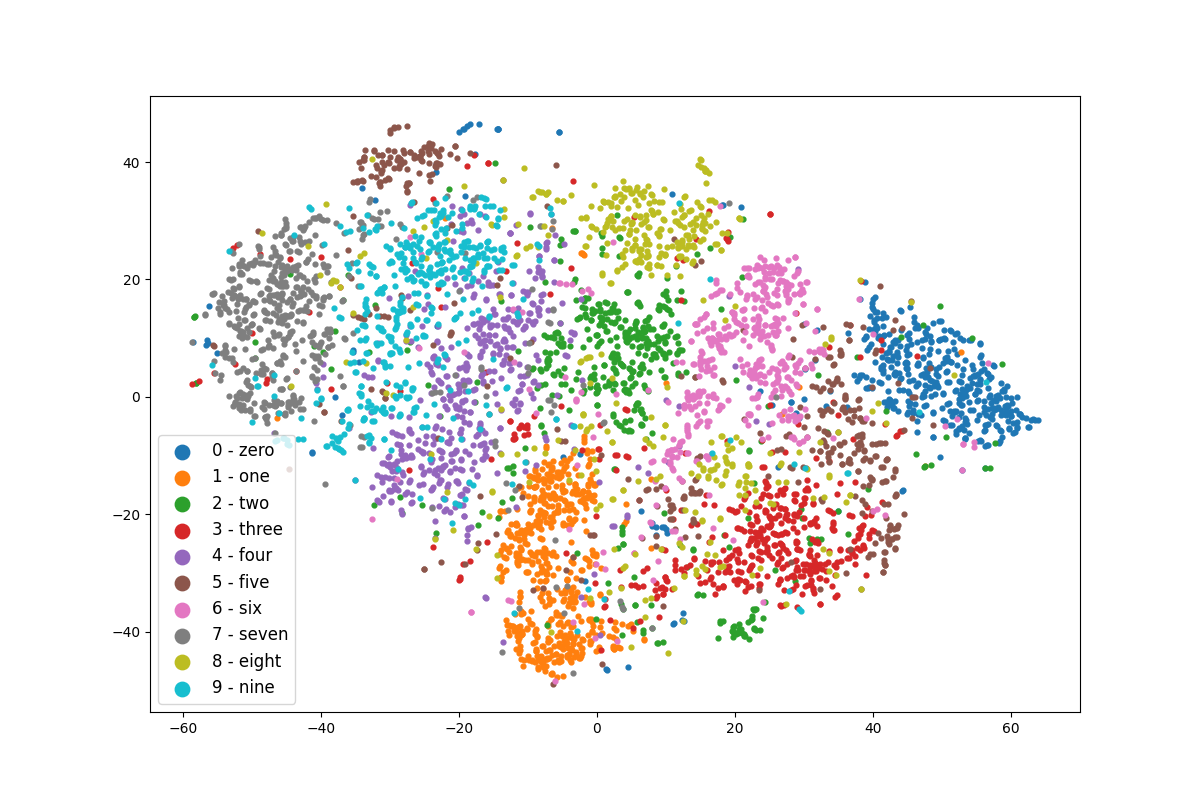
\includegraphics[width=1.0\textwidth]{../../out/activations_cnn/mnist/t-sne/untrained/plot_l2_f0.png}
    \caption{Embeddings of activations in the second layer of an untrained neural network (t-SNE).}
\end{figure}

\begin{figure}
  \centering
    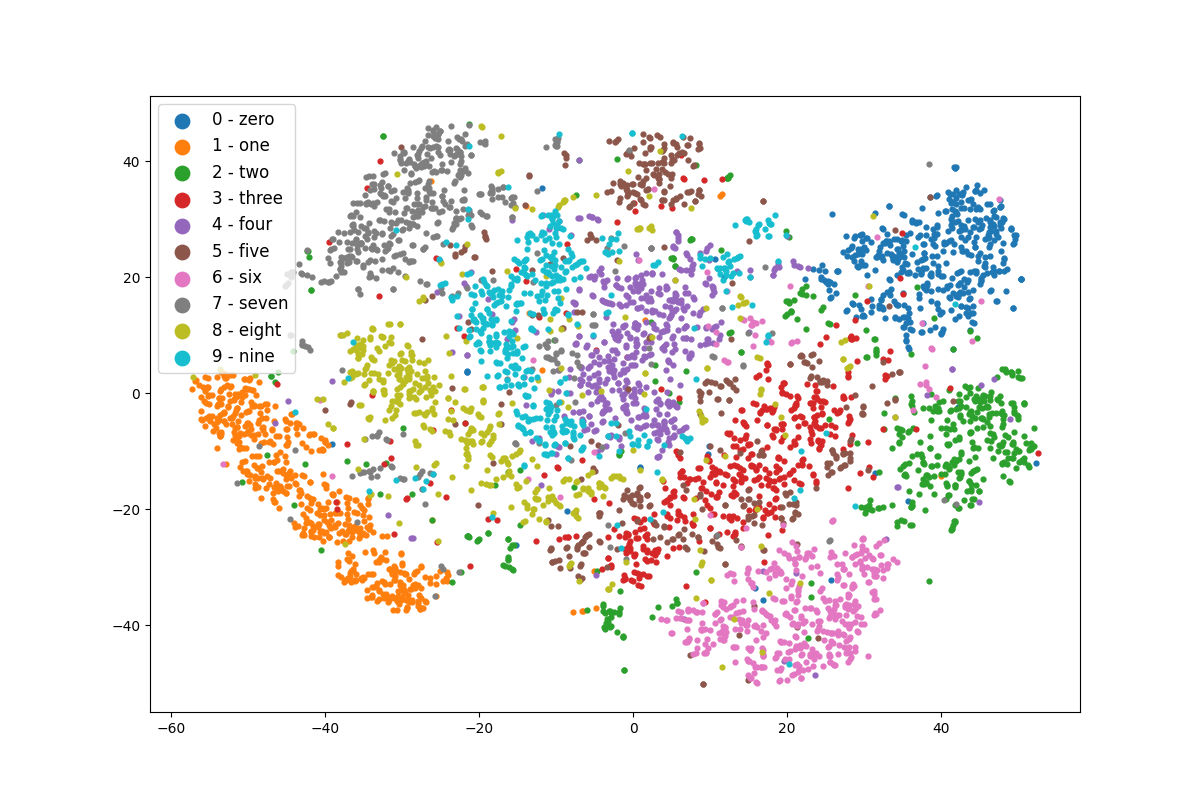
\includegraphics[width=1.0\textwidth]{../../out/activations_cnn/mnist/t-sne/untrained/plot_l3.png}
    \caption{Embeddings of activations in the third layer of an untrained neural network (t-SNE).}
\end{figure}

We might make an interesting observation - in the trained neural network, the
representations don't seem to get simply better the deeper the layer is.
Representations in the third layer seem to be the best (in terms of distances
between examples of same / different class), but representations in the second
and third layer seem to be worse than representations for the original
dataset. This could be explained by the fact that a lot of information can
be lost by applying a filter to an image; combining the outputs of
the filters should then result in greater embedding quality. This would
suggest that computing an average of values of individual metrics over
the whole layer might not be the best way to actually evaluate the
quality of embeddings for the whole layer; how that could be done is
out of the scope of this work.

The representations obtained from the untrained network follow the same
pattern with two important distinctions:
\begin{enumerate}
  \item The representations are generally better in the trained network.
  \item The representation quality is worse in the third layer of an
      untrained neural network than it is in the case of the original
      dataset; the opposite holds in the case of the trained network.
\end{enumerate}

Plotting the embeddings gives us a rough idea of the quality of the
embeddings. However, we would also like to see values of metrics
introduced in the previous section. Figures 8 to 11 present tables
with values of those metrics. There are two values per layer and metric - the
first one corresponds to the trained network, the second one to the untrained
network. As it is not very easy to see what is the general trend in these
values, we also provide plots with average values of metrics in each layer.
We only provide plots for the \(d_s\) and \(d_d\) metrics for lack of space;
however, the same trend can be observed in the rest of the metrics too.
Figures 12 and 13 contain these plots.

\begin{figure}
  \centering
    \resizebox{\textwidth}{!}{
        \begin{tabular}{llllll}
\toprule
{} &               ds &               dd &               cs &               cd &          acc\_knn \\
\midrule
filter 1 &  0.3773 / 0.3773 &  1.0695 / 1.0695 &  0.2664 / 0.2664 &  0.9748 / 0.9748 &  0.9398 / 0.9398 \\
\bottomrule
\end{tabular}

    }
  \caption{Values of metrics for embeddings acquired by t-SNE, original dataset.}
\end{figure}

\begin{figure}
  \centering
    \resizebox{\textwidth}{!}{
        \begin{tabular}{llllll}
\toprule
{} &               ds &               dd &               cs &               cd &          acc\_knn \\
\midrule
filter 1 &  0.3550 / 0.4218 &  1.0720 / 1.0645 &  0.2589 / 0.3085 &  0.9758 / 0.9486 &  0.9340 / 0.9328 \\
filter 2 &  0.3771 / 0.3643 &  1.0695 / 1.0709 &  0.2714 / 0.2612 &  0.9805 / 0.9761 &  0.9472 / 0.9428 \\
filter 3 &  0.3316 / 0.3296 &  1.0746 / 1.0748 &  0.2351 / 0.2346 &  0.9958 / 0.9952 &  0.9394 / 0.9448 \\
filter 4 &  0.4326 / 0.4920 &  1.0633 / 1.0567 &  0.3155 / 0.3670 &  0.9331 / 0.8796 &  0.9214 / 0.8996 \\
\bottomrule
\end{tabular}

    }
    \caption{Values of metrics for embeddings acquired by t-SNE, first layer.}
\end{figure}

\begin{figure}
  \centering
    \resizebox{\textwidth}{!}{
        \begin{tabular}{llllll}
\toprule
{} &               ds &               dd &               cs &               cd &          acc\_knn \\
\midrule
filter 1  &  0.4455 / 0.5469 &  1.0619 / 1.0506 &  0.3277 / 0.4174 &  0.9137 / 0.7944 &  0.8794 / 0.8224 \\
filter 2  &  0.5410 / 0.6565 &  1.0512 / 1.0383 &  0.4017 / 0.4807 &  0.8445 / 0.7281 &  0.8516 / 0.7182 \\
filter 3  &  0.5855 / 0.5865 &  1.0463 / 1.0461 &  0.4330 / 0.4219 &  0.8116 / 0.8147 &  0.8442 / 0.8266 \\
filter 4  &  0.5770 / 0.4310 &  1.0472 / 1.0635 &  0.4264 / 0.3080 &  0.8110 / 0.9249 &  0.8512 / 0.8782 \\
filter 5  &  0.4406 / 0.5063 &  1.0624 / 1.0551 &  0.3176 / 0.3809 &  0.9215 / 0.8540 &  0.8920 / 0.8746 \\
filter 6  &  0.4279 / 0.4685 &  1.0638 / 1.0593 &  0.3054 / 0.3410 &  0.9402 / 0.9229 &  0.8794 / 0.8508 \\
filter 7  &  0.4393 / 0.4066 &  1.0626 / 1.0662 &  0.3081 / 0.2887 &  0.9218 / 0.9443 &  0.8798 / 0.8950 \\
filter 8  &  0.4219 / 0.5111 &  1.0645 / 1.0546 &  0.3107 / 0.3710 &  0.9338 / 0.8676 &  0.8882 / 0.7876 \\
filter 9  &  0.4777 / 0.4045 &  1.0583 / 1.0664 &  0.3469 / 0.2893 &  0.8954 / 0.9550 &  0.8532 / 0.8878 \\
filter 10 &  0.4539 / 0.8760 &  1.0609 / 1.0138 &  0.3256 / 0.6570 &  0.9248 / 0.4283 &  0.8688 / 0.4660 \\
filter 11 &  0.5357 / 0.7257 &  1.0518 / 1.0306 &  0.3995 / 0.5299 &  0.8440 / 0.6375 &  0.8642 / 0.6910 \\
filter 12 &  0.4215 / 0.7265 &  1.0646 / 1.0305 &  0.3121 / 0.5783 &  0.9274 / 0.6335 &  0.8992 / 0.4774 \\
filter 13 &  0.4534 / 0.6405 &  1.0610 / 1.0401 &  0.3194 / 0.4892 &  0.9305 / 0.7075 &  0.8568 / 0.8198 \\
filter 14 &  0.6861 / 0.5102 &  1.0350 / 1.0547 &  0.5150 / 0.3752 &  0.6828 / 0.8604 &  0.7858 / 0.8278 \\
filter 15 &  0.5404 / 0.6304 &  1.0513 / 1.0412 &  0.3984 / 0.4869 &  0.8416 / 0.7232 &  0.8630 / 0.8064 \\
filter 16 &  0.4875 / 0.5654 &  1.0572 / 1.0485 &  0.3595 / 0.4239 &  0.8901 / 0.8020 &  0.8736 / 0.8124 \\
\bottomrule
\end{tabular}

    }
    \caption{Values of metrics for embeddings acquired by t-SNE, second layer.}
\end{figure}

\begin{figure}
  \centering
    \resizebox{\textwidth}{!}{
        \begin{tabular}{llllll}
\toprule
{} &               ds &               dd &               cs &               cd &          acc\_knn \\
\midrule
filter 1 &  0.2370 / 0.5046 &  1.0851 / 1.0553 &  0.1678 / 0.3772 &  1.0544 / 0.8534 &  0.9854 / 0.8654 \\
\bottomrule
\end{tabular}

    }
    \caption{Values of metrics for embeddings acquired by t-SNE, third layer.}
\end{figure}

\begin{figure}
  \centering
    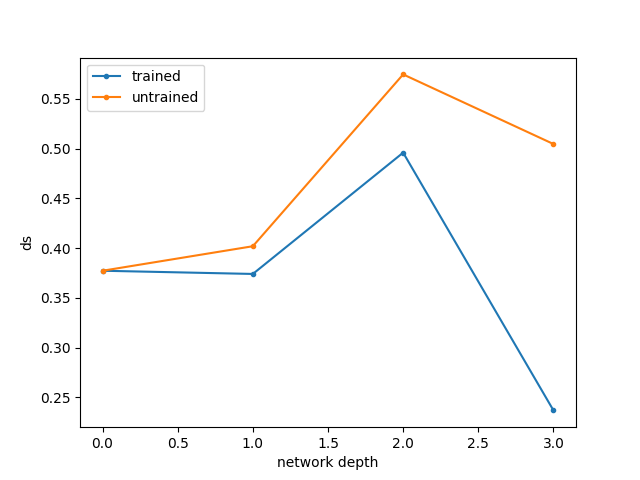
\includegraphics[width=0.75\textwidth]{../../out/activations_cnn/mnist/t-sne/plot_metric_ds.png}
    \caption{Average value of the \(d_s\) metric (t-SNE).}
\end{figure}

\begin{figure}
  \centering
    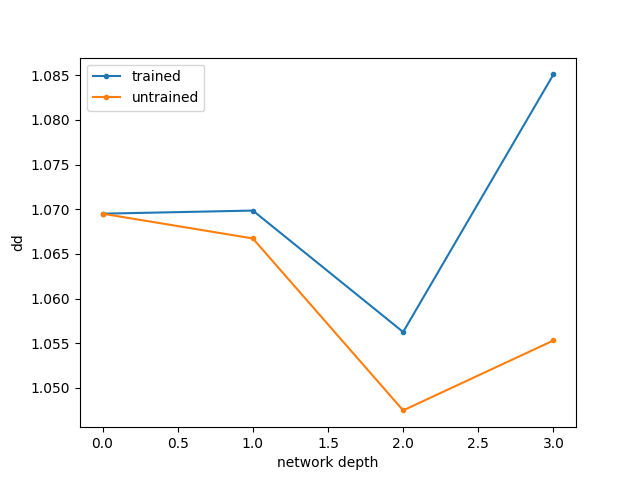
\includegraphics[width=0.75\textwidth]{../../out/activations_cnn/mnist/t-sne/plot_metric_dd.png}
    \caption{Average value of the \(d_d\) metric (t-SNE).}
\end{figure}

The trend we are seeing both from the tables and from the plots is the same
one we noted when inspecting the embeddings visually.

Even the representations in the third layer of the trained neural network
seem to contain some outliers - points that our in a wrong cluster. For
example, we might notice that there are several examples with true label
3 in the cluster of examples labeled 7. One such example can be seen in
Figure 14.

\begin{figure}
  \centering
  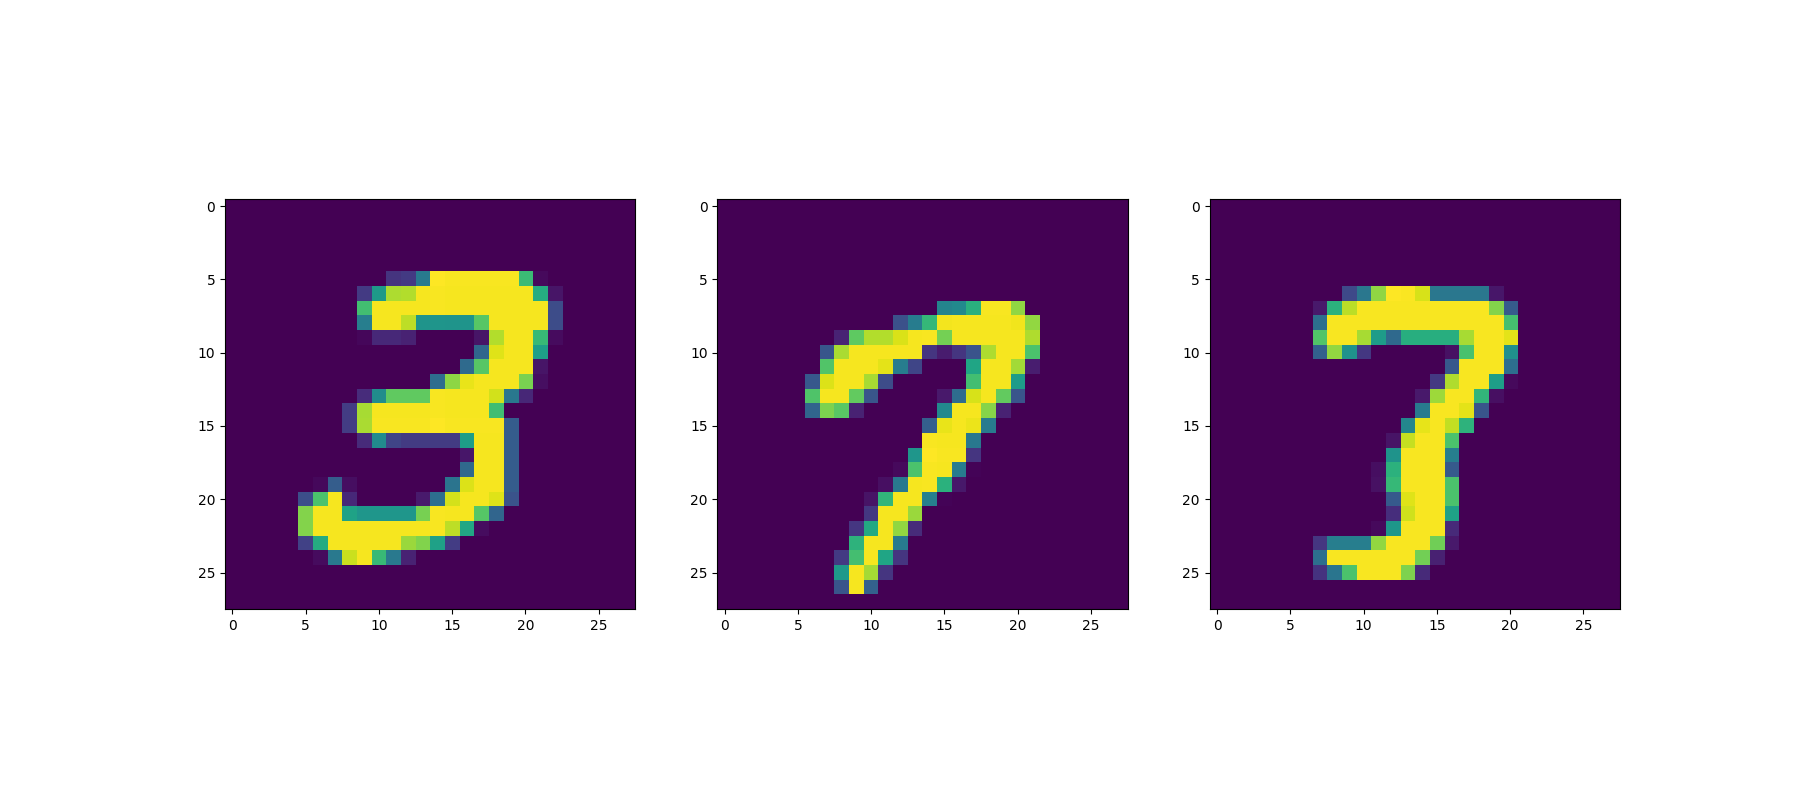
\includegraphics[width=0.75\textwidth]{../../out/activations_cnn/mnist/t-sne/outliers/correct3_predicted7.png}
    \caption{From left: an example of 3, an example of 7, the missclasified example.}
\end{figure}

The figure also contains two other examples, which show what an average
example of 3 and 7 looks like. What we might notice is that the outlier
does seem to contain features characteristic for both 3 and 7 and it
might not be immediately clear, even to a human, what number it really
is.

It might also be of interest to us what do the individual filters do.
Figures 15 to 17 visualize the activations of the network for an example
from the dataset. 

\begin{figure}
  \centering
  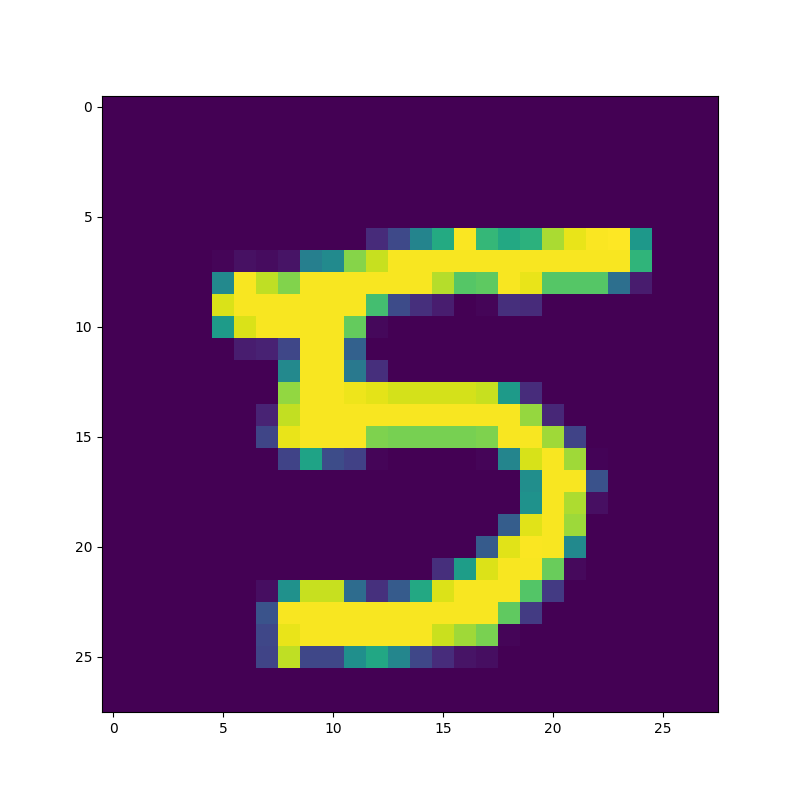
\includegraphics[width=0.75\textwidth]{../../out/activations_cnn/mnist/t-sne/filter_outputs/class5_l0.png}
    \caption{An example of 5.}
\end{figure}

\begin{figure}
  \centering
  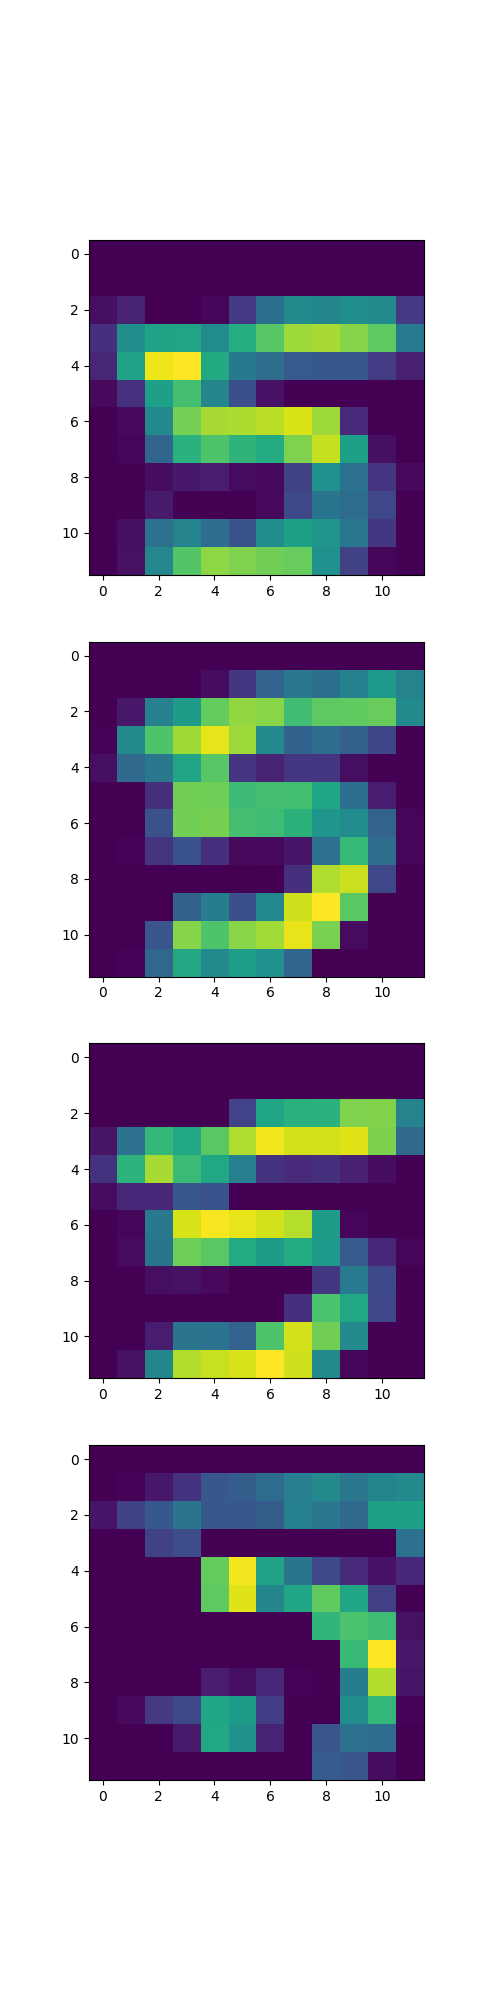
\includegraphics[width=0.25\textwidth]{../../out/activations_cnn/mnist/t-sne/filter_outputs/class5_l1.png}
  \caption{Activations in the first layer of the network for the example.}
\end{figure}

\begin{figure}
  \centering
  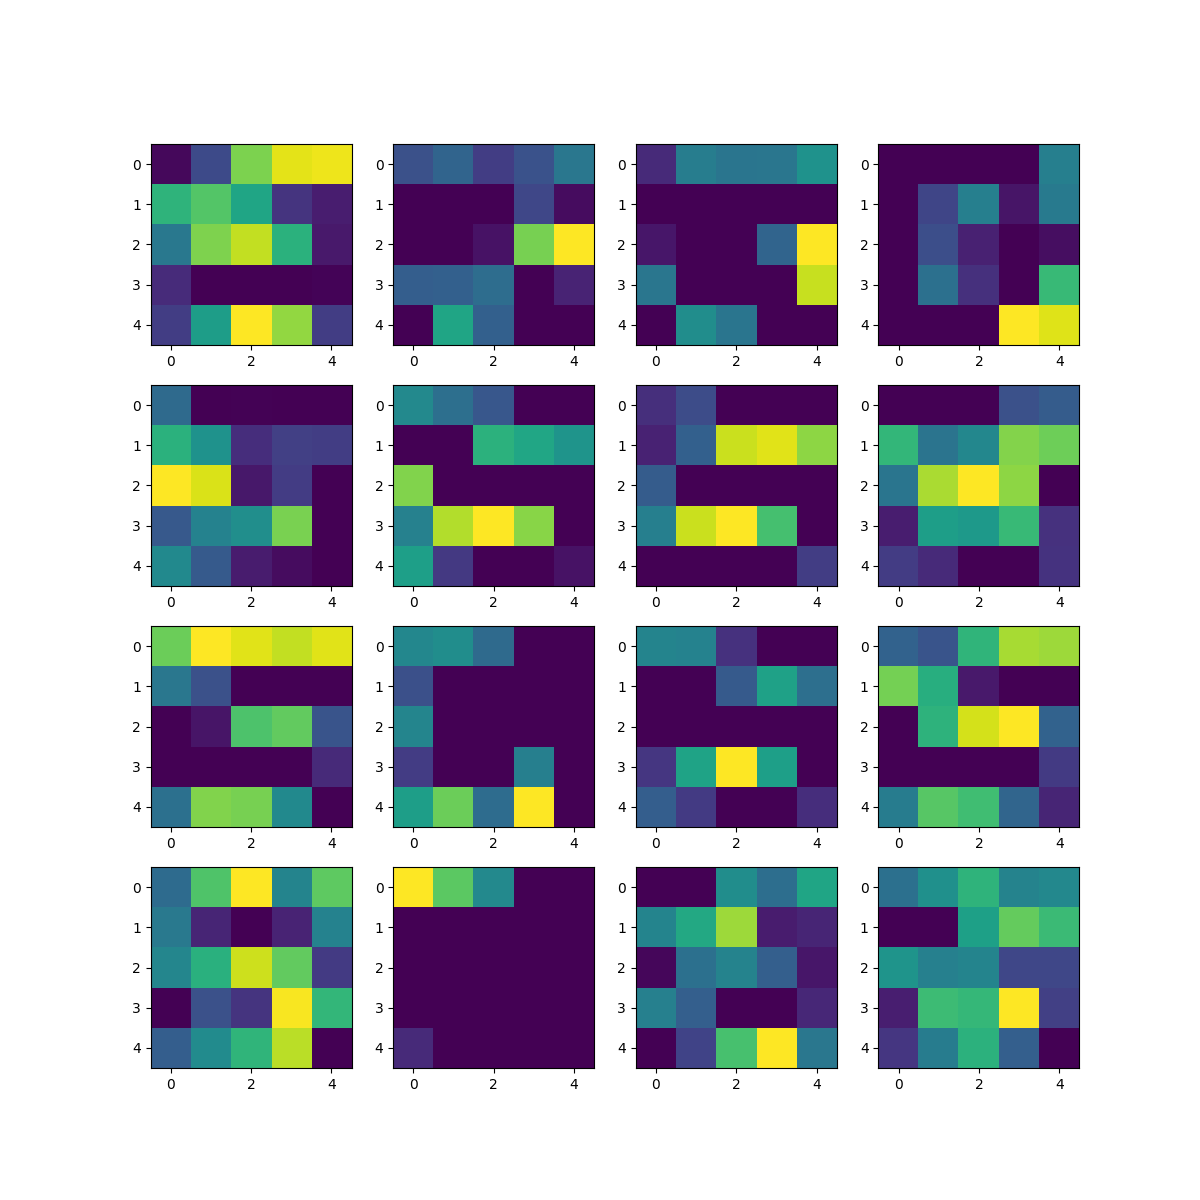
\includegraphics[width=0.75\textwidth]{../../out/activations_cnn/mnist/t-sne/filter_outputs/class5_l2.png}
    \caption{Activations in the second layer of the network for the example.}
\end{figure}

In the first layer, it seems that the first and third filter detects some
variation of a horizontal line, and it also seems that the second and fourth
filter detects some variation of a diagonal line. The activations in the
second layer are not as easy to analyze and it is not clear what purpose each
filter serves.

Using UMAP to acquire embeddings, we get very similar results. Figures 18
to 24 show the computed embeddings.

\begin{figure}
  \centering
    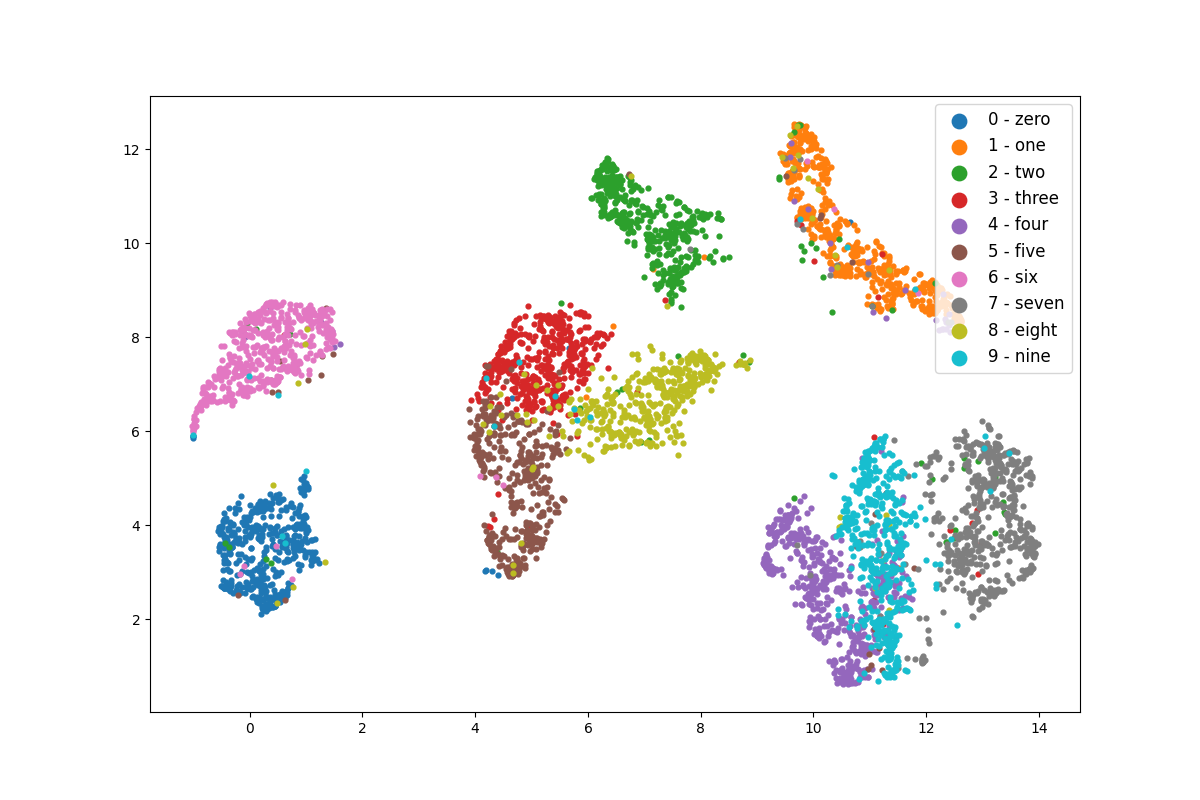
\includegraphics[width=1.0\textwidth]{../../out/activations_cnn/mnist/umap/trained/plot_l0.png}
    \caption{Embeddings of the original dataset (UMAP).}
\end{figure}

\begin{figure}
  \centering
    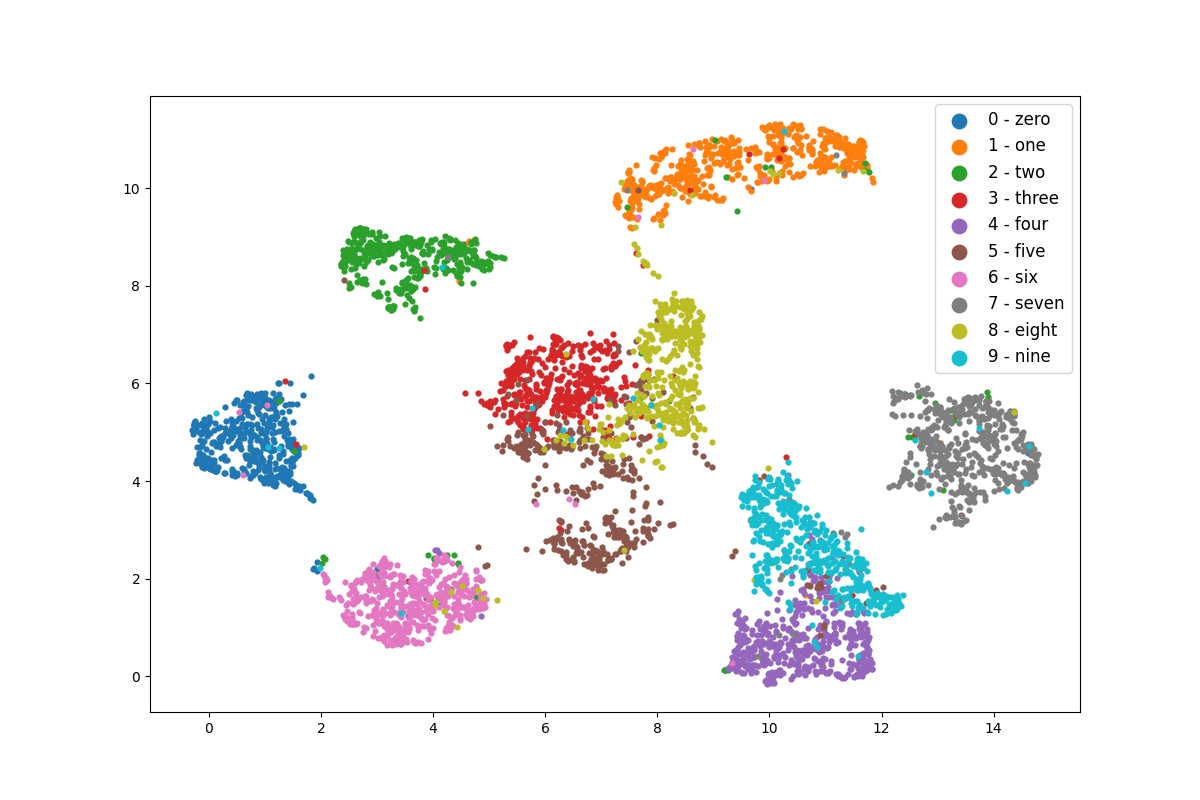
\includegraphics[width=1.0\textwidth]{../../out/activations_cnn/mnist/umap/trained/plot_l1_f0.png}
    \caption{Embeddings of activations in the first layer of a neural network trained on MNIST (UMAP).}
\end{figure}

\begin{figure}
  \centering
    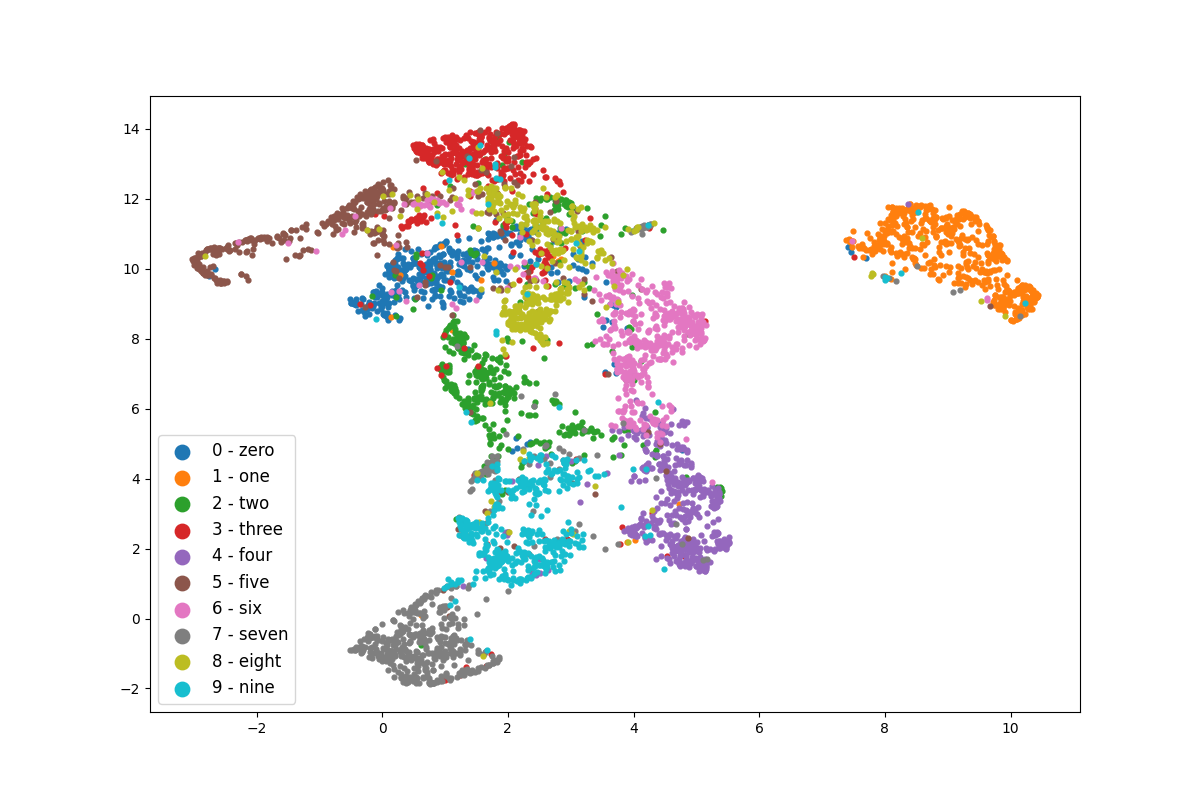
\includegraphics[width=1.0\textwidth]{../../out/activations_cnn/mnist/umap/trained/plot_l2_f0.png}
    \caption{Embeddings of activations in the second layer of a neural network trained on MNIST (UMAP).}
\end{figure}

\begin{figure}
  \centering
    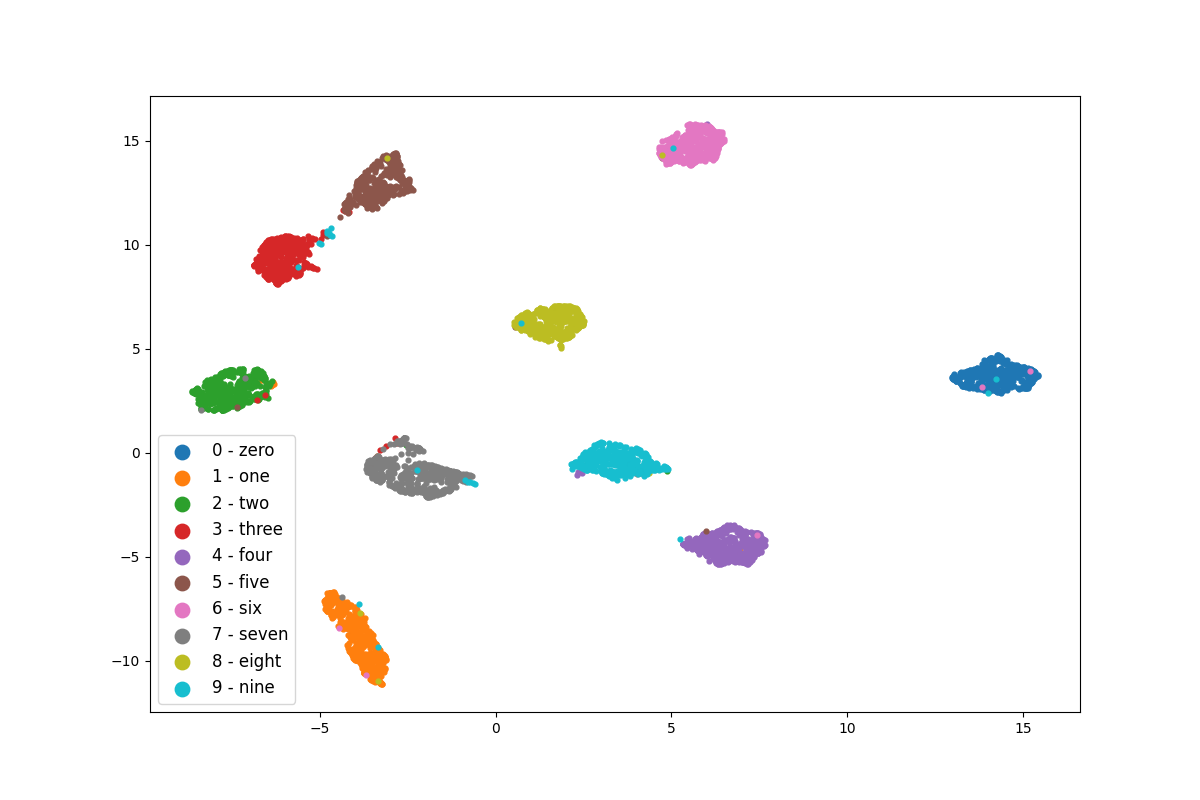
\includegraphics[width=1.0\textwidth]{../../out/activations_cnn/mnist/umap/trained/plot_l3.png}
    \caption{Embeddings of activations in the third layer of a neural network trained on MNIST (UMAP).}
\end{figure}

\begin{figure}
  \centering
    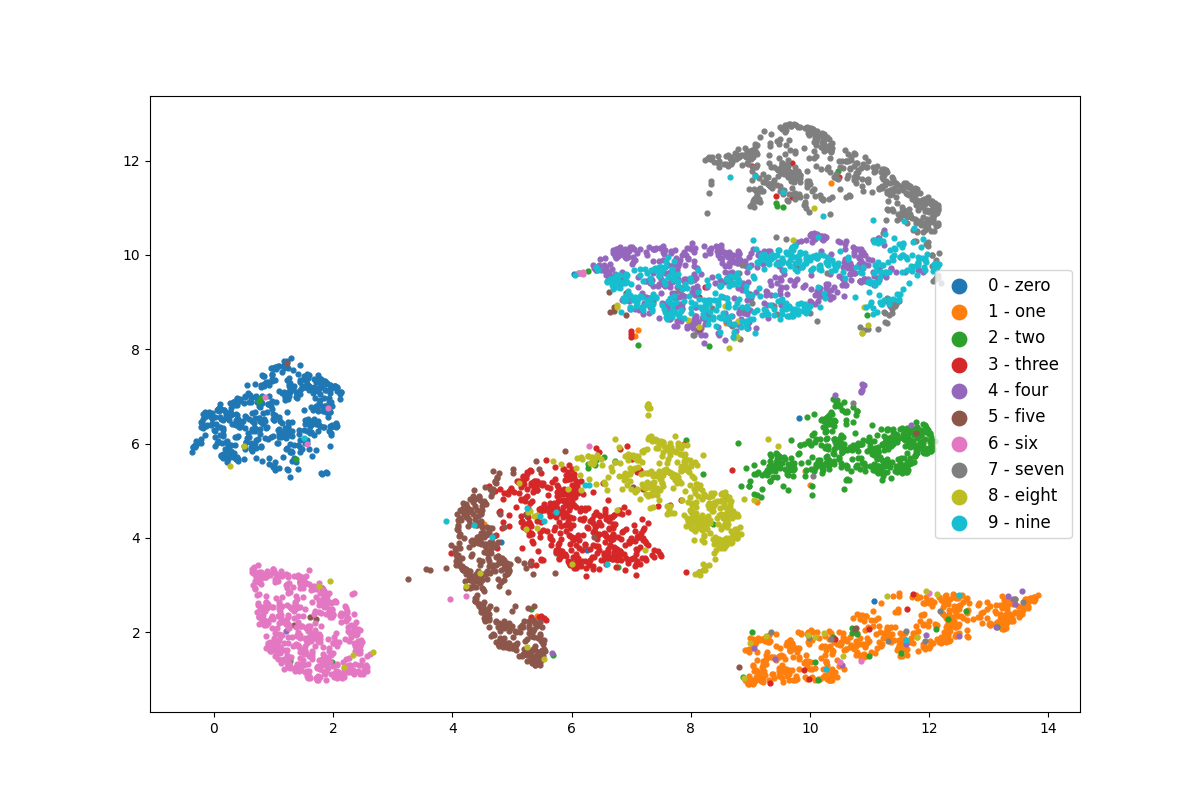
\includegraphics[width=1.0\textwidth]{../../out/activations_cnn/mnist/umap/untrained/plot_l1_f0.png}
    \caption{Embeddings of activations in the first layer of an untrained neural network (UMAP).}
\end{figure}

\begin{figure}
  \centering
    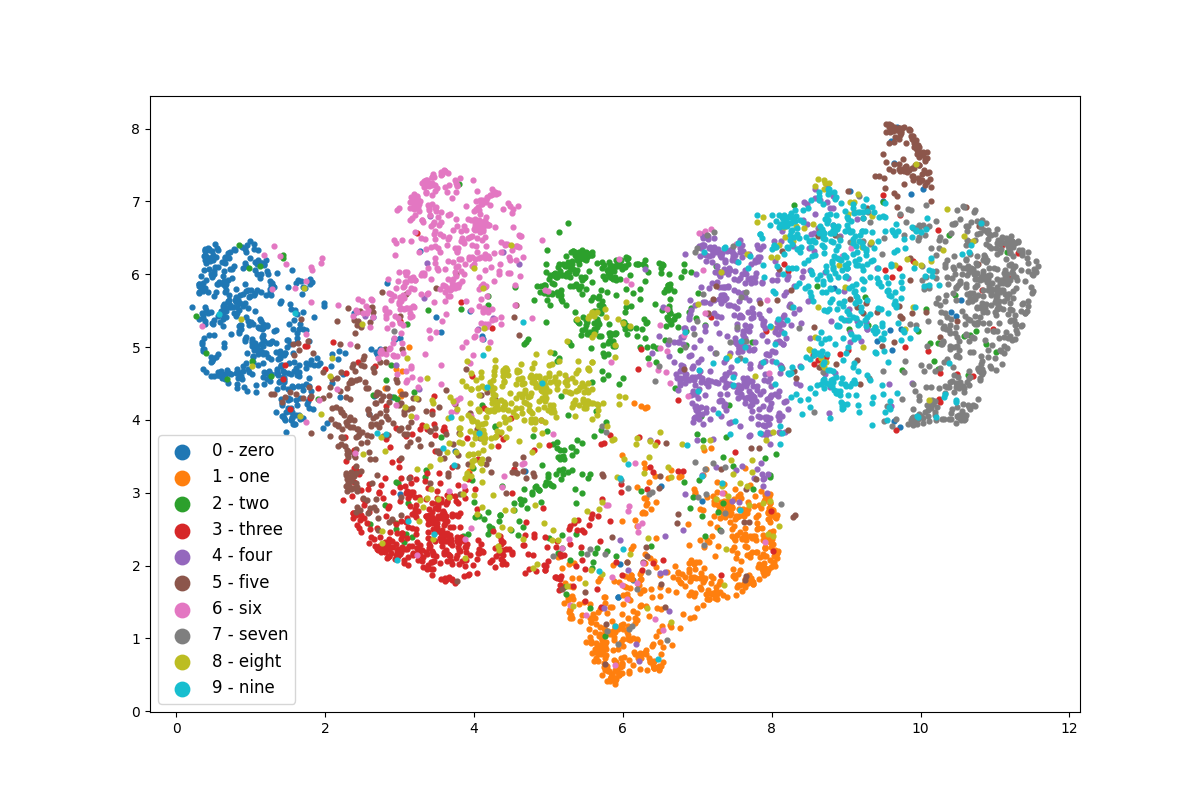
\includegraphics[width=1.0\textwidth]{../../out/activations_cnn/mnist/umap/untrained/plot_l2_f0.png}
    \caption{Embeddings of activations in the second layer of an untrained neural network (UMAP).}
\end{figure}

\begin{figure}
  \centering
    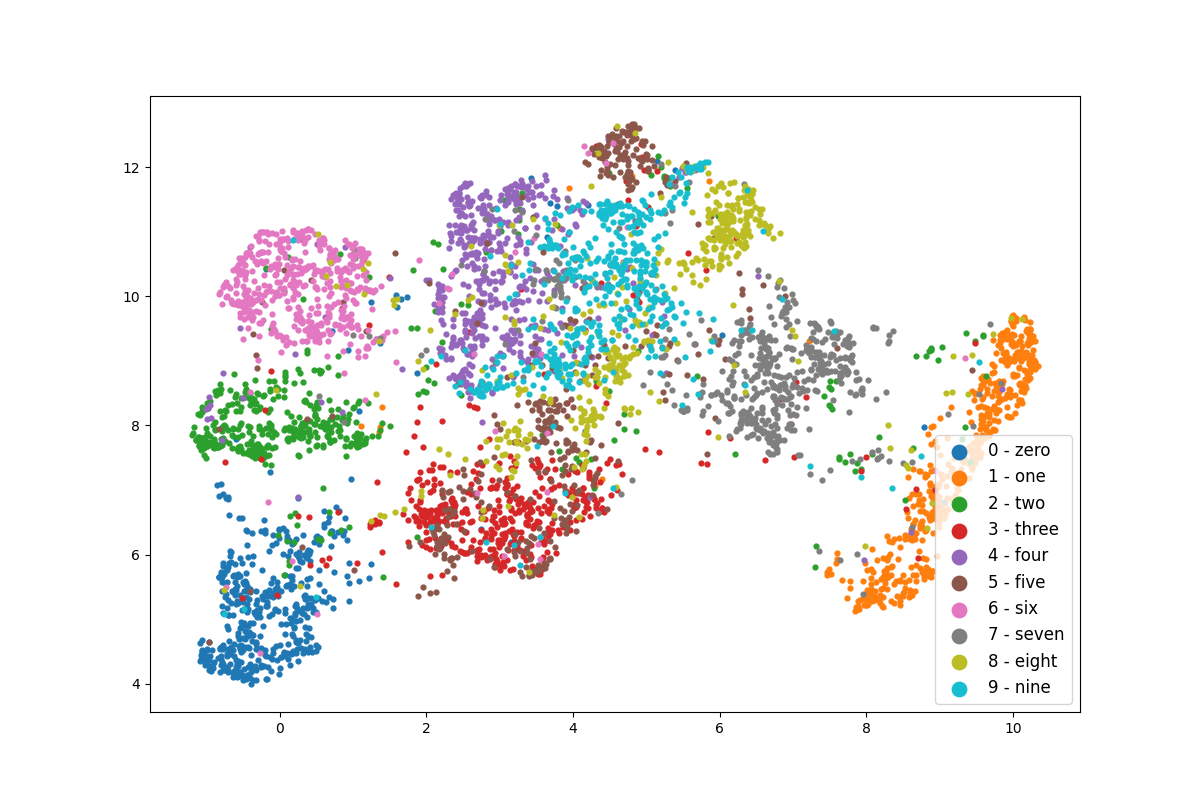
\includegraphics[width=1.0\textwidth]{../../out/activations_cnn/mnist/umap/untrained/plot_l3.png}
    \caption{Embeddings of activations in the third layer of an untrained neural network (UMAP).}
\end{figure}

Again, we would like to confirm our observations by comparing values of
metrics over the computed embeddings. These can be seen in Figures 25 to
30.

\begin{figure}
  \centering
    \resizebox{\textwidth}{!}{
        \begin{tabular}{llllll}
\toprule
{} &               ds &               dd &               cs &               cd &          acc\_knn \\
\midrule
filter 1 &  0.2759 / 0.2721 &  1.0808 / 1.0812 &  0.1921 / 0.1894 &  1.0125 / 1.0146 &  0.9268 / 0.9396 \\
\bottomrule
\end{tabular}

    }
  \caption{Values of metrics for embeddings acquired by UMAP, original dataset.}
\end{figure}

\begin{figure}
  \centering
    \resizebox{\textwidth}{!}{
        \begin{tabular}{llllll}
\toprule
{} &               ds &               dd &               cs &               cd &          acc\_knn \\
\midrule
filter 1 &  0.2682 / 0.2983 &  1.0817 / 1.0783 &  0.1902 / 0.2089 &  1.0118 / 1.0004 &  0.9278 / 0.9028 \\
filter 2 &  0.2397 / 0.2550 &  1.0848 / 1.0831 &  0.1682 / 0.1776 &  1.0326 / 1.0227 &  0.9492 / 0.9434 \\
filter 3 &  0.2601 / 0.2325 &  1.0826 / 1.0856 &  0.1814 / 0.1625 &  1.0226 / 1.0339 &  0.9296 / 0.9350 \\
filter 4 &  0.3193 / 0.3608 &  1.0760 / 1.0713 &  0.2261 / 0.2589 &  1.0041 / 0.9694 &  0.8956 / 0.8800 \\
\bottomrule
\end{tabular}

    }
    \caption{Values of metrics for embeddings acquired by UMAP, first layer.}
\end{figure}

\begin{figure}
  \centering
    \resizebox{\textwidth}{!}{
        \begin{tabular}{llllll}
\toprule
{} &               ds &               dd &               cs &               cd &          acc\_knn \\
\midrule
filter 1  &  0.3678 / 0.4829 &  1.0705 / 1.0577 &  0.2664 / 0.3686 &  0.9489 / 0.8499 &  0.8736 / 0.7978 \\
filter 2  &  0.5066 / 0.6238 &  1.0551 / 1.0420 &  0.3776 / 0.4587 &  0.8616 / 0.7358 &  0.8182 / 0.6976 \\
filter 3  &  0.4963 / 0.5375 &  1.0562 / 1.0516 &  0.3586 / 0.3827 &  0.8764 / 0.8453 &  0.8196 / 0.7820 \\
filter 4  &  0.5073 / 0.3684 &  1.0550 / 1.0705 &  0.3638 / 0.2636 &  0.8848 / 0.9623 &  0.7918 / 0.8422 \\
filter 5  &  0.3663 / 0.4185 &  1.0707 / 1.0649 &  0.2597 / 0.3025 &  0.9701 / 0.9230 &  0.8814 / 0.8440 \\
filter 6  &  0.3964 / 0.4408 &  1.0674 / 1.0624 &  0.2839 / 0.3222 &  0.9544 / 0.9276 &  0.8694 / 0.8250 \\
filter 7  &  0.4176 / 0.3447 &  1.0650 / 1.0731 &  0.2937 / 0.2397 &  0.9295 / 0.9661 &  0.8600 / 0.8856 \\
filter 8  &  0.3533 / 0.4895 &  1.0722 / 1.0570 &  0.2497 / 0.3506 &  0.9644 / 0.8867 &  0.8816 / 0.7530 \\
filter 9  &  0.4221 / 0.3705 &  1.0645 / 1.0702 &  0.3009 / 0.2604 &  0.9351 / 0.9663 &  0.8312 / 0.8516 \\
filter 10 &  0.4524 / 0.8812 &  1.0611 / 1.0133 &  0.3244 / 0.6720 &  0.9181 / 0.4235 &  0.8534 / 0.4684 \\
filter 11 &  0.4570 / 0.6986 &  1.0606 / 1.0336 &  0.3371 / 0.5102 &  0.9120 / 0.6830 &  0.8444 / 0.6626 \\
filter 12 &  0.3639 / 0.7084 &  1.0710 / 1.0325 &  0.2654 / 0.5821 &  0.9553 / 0.6493 &  0.8930 / 0.4898 \\
filter 13 &  0.4148 / 0.5297 &  1.0653 / 1.0525 &  0.2965 / 0.3886 &  0.9470 / 0.8504 &  0.8350 / 0.7884 \\
filter 14 &  0.6577 / 0.4621 &  1.0382 / 1.0600 &  0.4898 / 0.3369 &  0.7099 / 0.8882 &  0.7464 / 0.7920 \\
filter 15 &  0.4817 / 0.5614 &  1.0578 / 1.0489 &  0.3511 / 0.4265 &  0.8936 / 0.8036 &  0.8394 / 0.7754 \\
filter 16 &  0.4008 / 0.4948 &  1.0669 / 1.0564 &  0.2897 / 0.3583 &  0.9410 / 0.8692 &  0.8596 / 0.7852 \\
\bottomrule
\end{tabular}

    }
    \caption{Values of metrics for embeddings acquired by UMAP, second layer.}
\end{figure}

\begin{figure}
  \centering
    \resizebox{\textwidth}{!}{
        \begin{tabular}{llllll}
\toprule
{} &               ds &               dd &               cs &               cd &          acc\_knn \\
\midrule
filter 1 &  0.1172 / 0.4456 &  1.0985 / 1.0619 &  0.0799 / 0.3288 &  1.0819 / 0.8912 &  0.9834 / 0.8310 \\
\bottomrule
\end{tabular}

    }
    \caption{Values of metrics for embeddings acquired by UMAP, third layer.}
\end{figure}

\begin{figure}
  \centering
    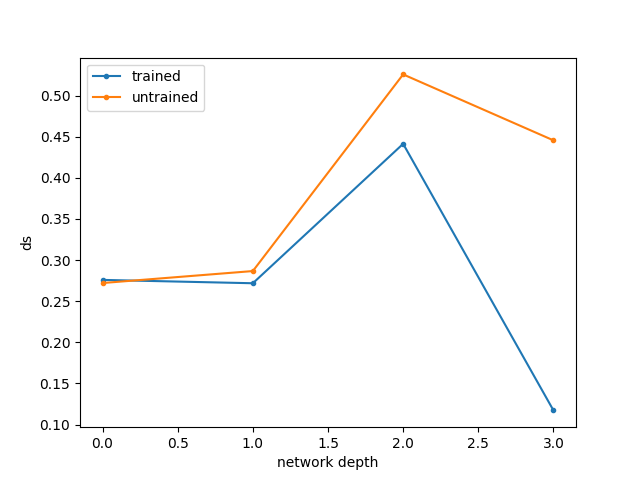
\includegraphics[width=0.75\textwidth]{../../out/activations_cnn/mnist/umap/plot_metric_ds.png}
    \caption{Average value of the \(d_s\) metric (UMAP).}
\end{figure}

\begin{figure}
  \centering
    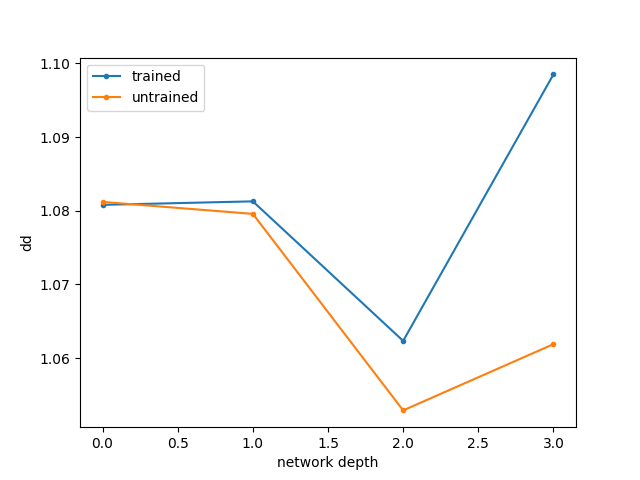
\includegraphics[width=0.75\textwidth]{../../out/activations_cnn/mnist/umap/plot_metric_dd.png}
    \caption{Average value of the \(d_d\) metric (UMAP).}
\end{figure}

Again, the trend we are seeing both from the tables and from the plots is the
same one we noted when inspecting the embeddings visually.

\subsection{FashionMNIST}
Again, we start by looking at embeddings produced by t-SNE. A single embedding
is shown per layer of the network in Figures 31 to 37.

\begin{figure}
  \centering
    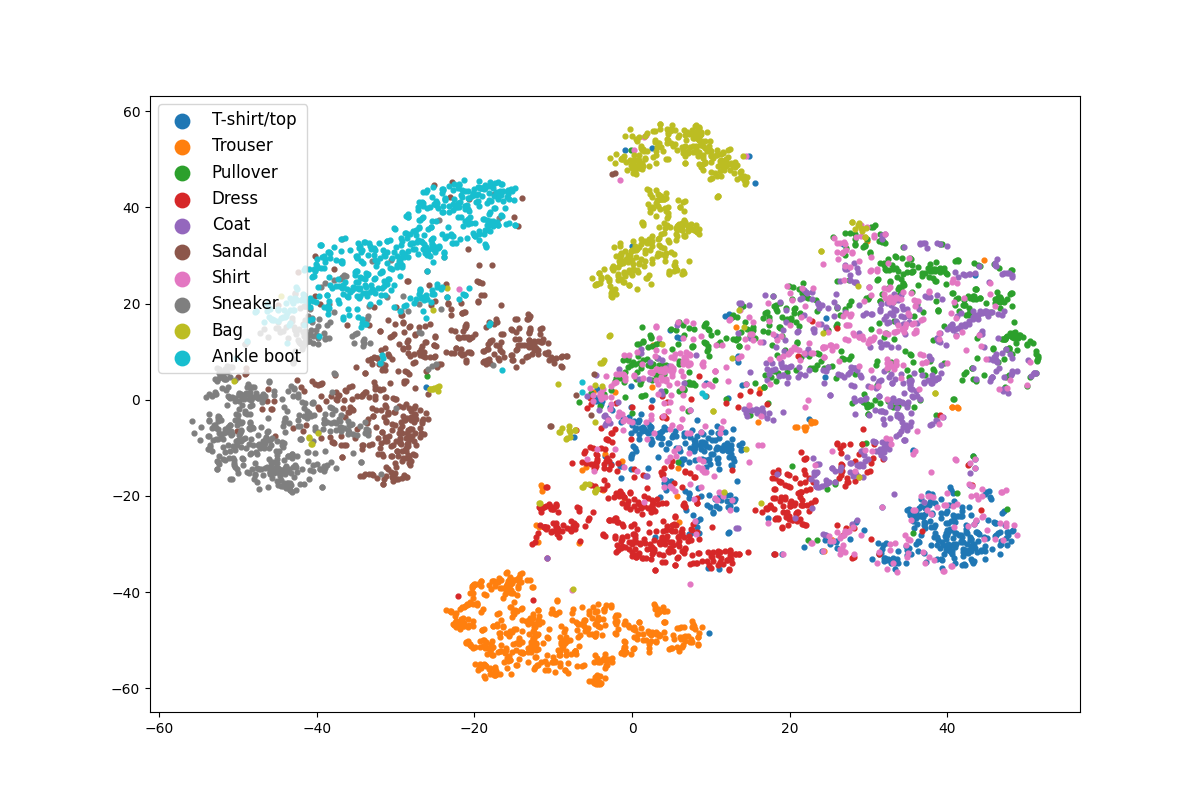
\includegraphics[width=1.0\textwidth]{../../out/activations_cnn/fmnist/t-sne/trained/plot_l0.png}
    \caption{Embeddings of the original dataset (t-SNE).}
\end{figure}

\begin{figure}
  \centering
    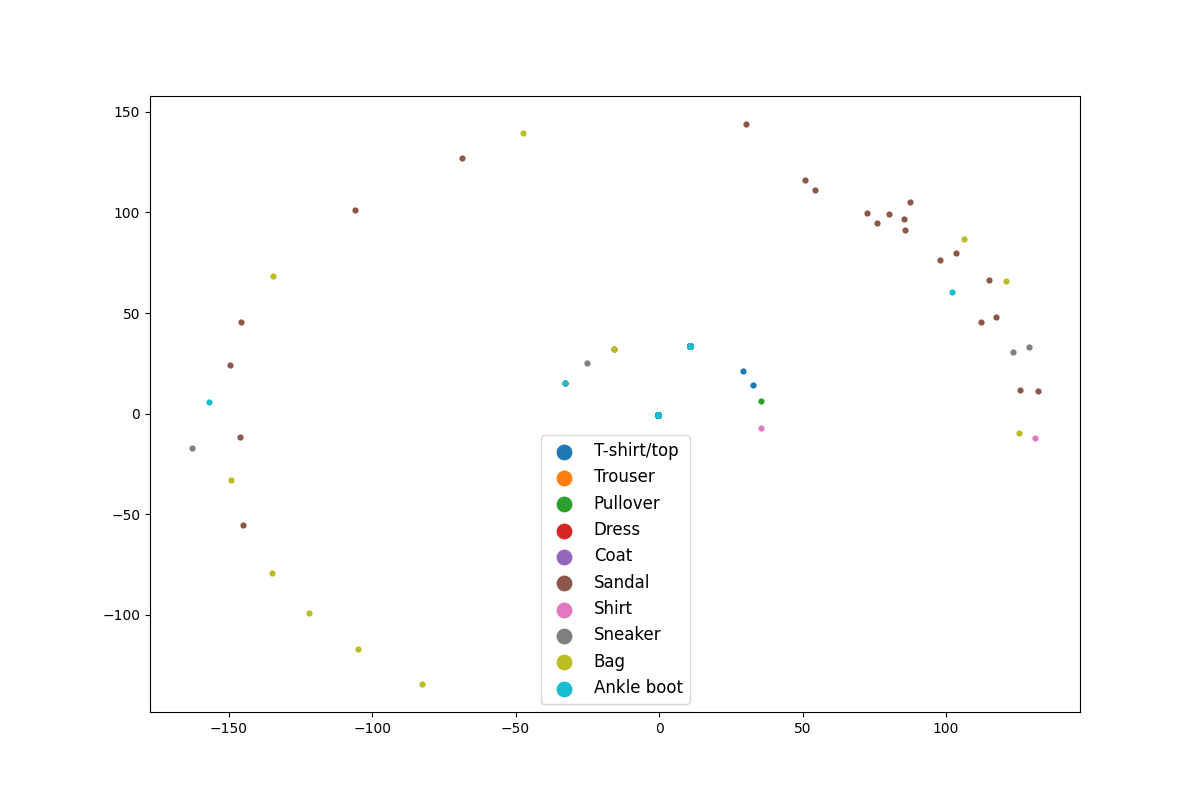
\includegraphics[width=1.0\textwidth]{../../out/activations_cnn/fmnist/t-sne/trained/plot_l1_f0.png}
    \caption{Embeddings of activations in the first layer of a neural network trained on FashionMNIST (t-SNE).}
\end{figure}

\begin{figure}
  \centering
    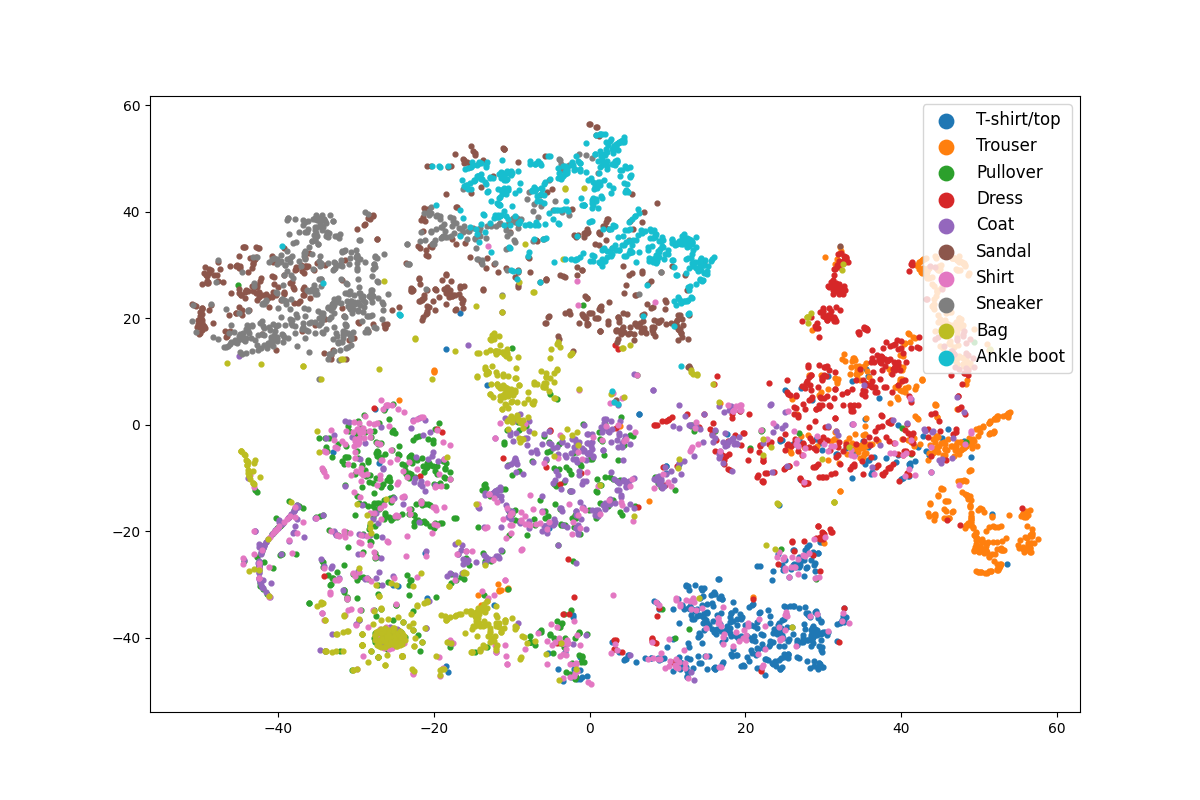
\includegraphics[width=1.0\textwidth]{../../out/activations_cnn/fmnist/t-sne/trained/plot_l2_f0.png}
    \caption{Embeddings of activations in the second layer of a neural network trained on FashionMNIST (t-SNE).}
\end{figure}

\begin{figure}
  \centering
    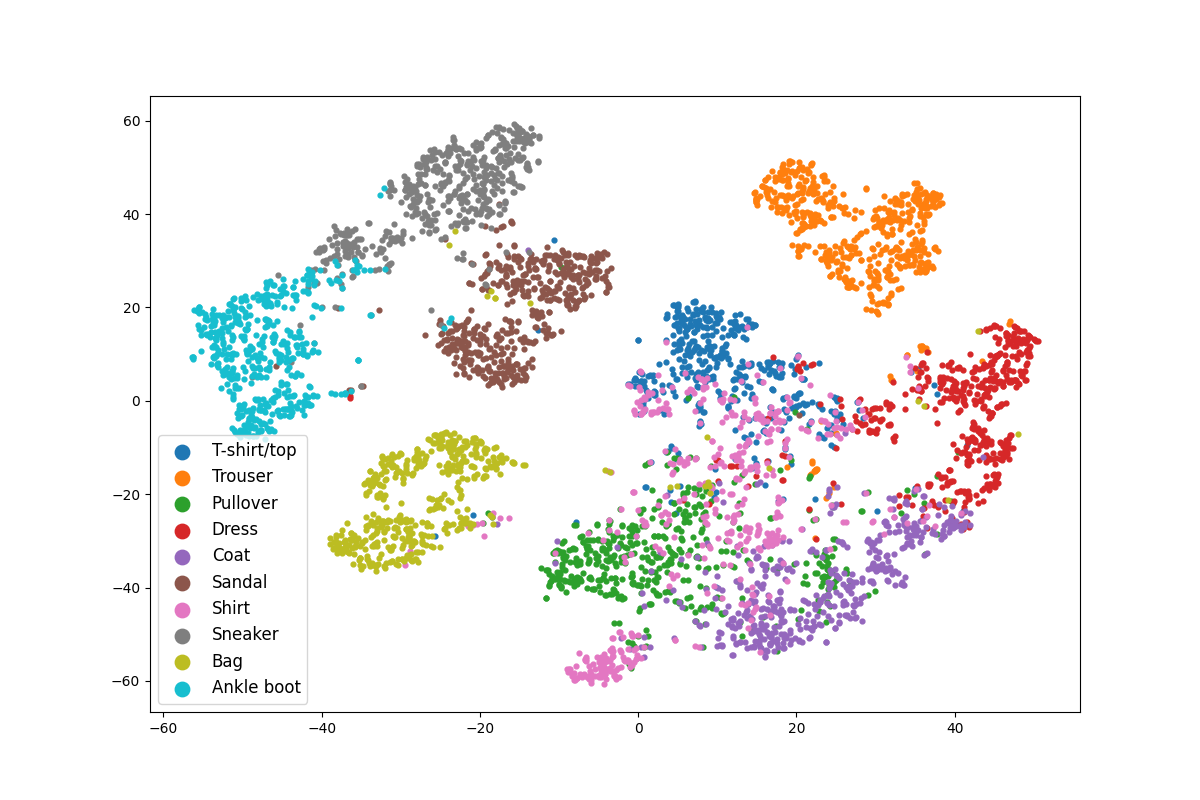
\includegraphics[width=1.0\textwidth]{../../out/activations_cnn/fmnist/t-sne/trained/plot_l3.png}
    \caption{Embeddings of activations in the third layer of a neural network trained on FashionMNIST (t-SNE).}
\end{figure}

\begin{figure}
  \centering
    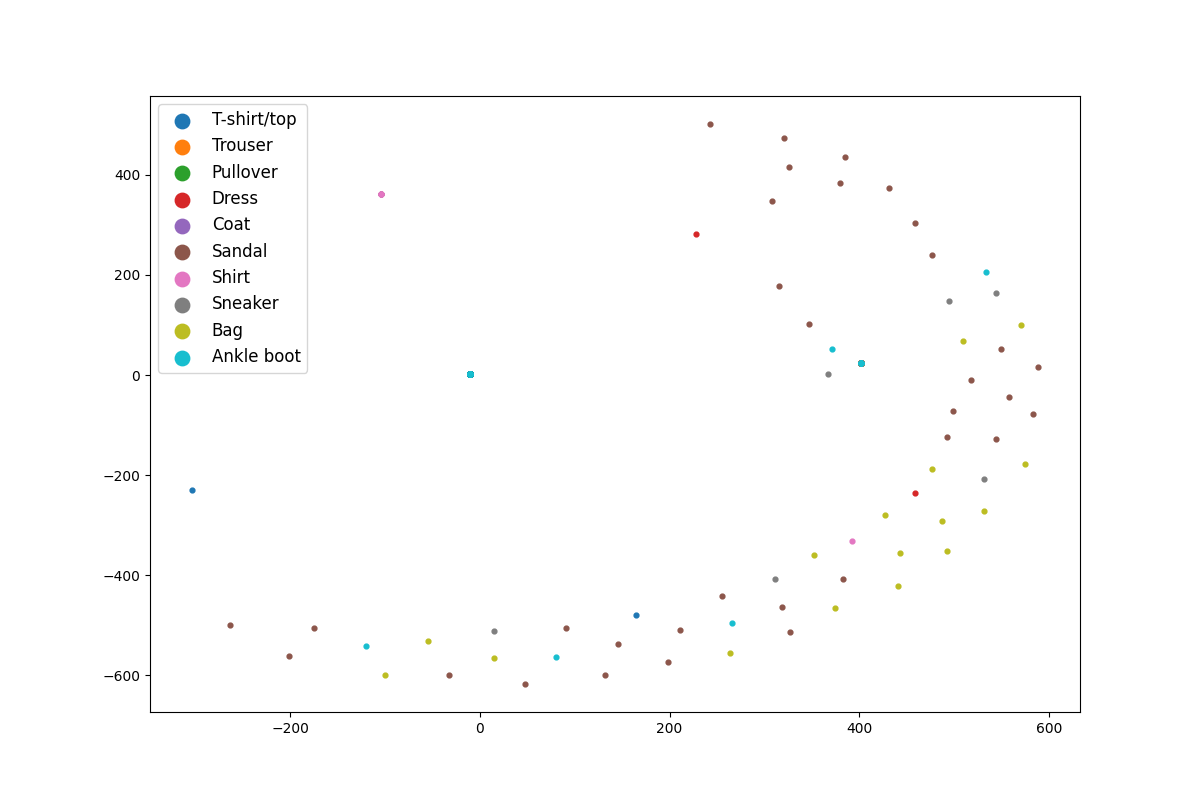
\includegraphics[width=1.0\textwidth]{../../out/activations_cnn/fmnist/t-sne/untrained/plot_l1_f0.png}
    \caption{Embeddings of activations in the first layer of an untrained neural network (t-SNE).}
\end{figure}

\begin{figure}
  \centering
    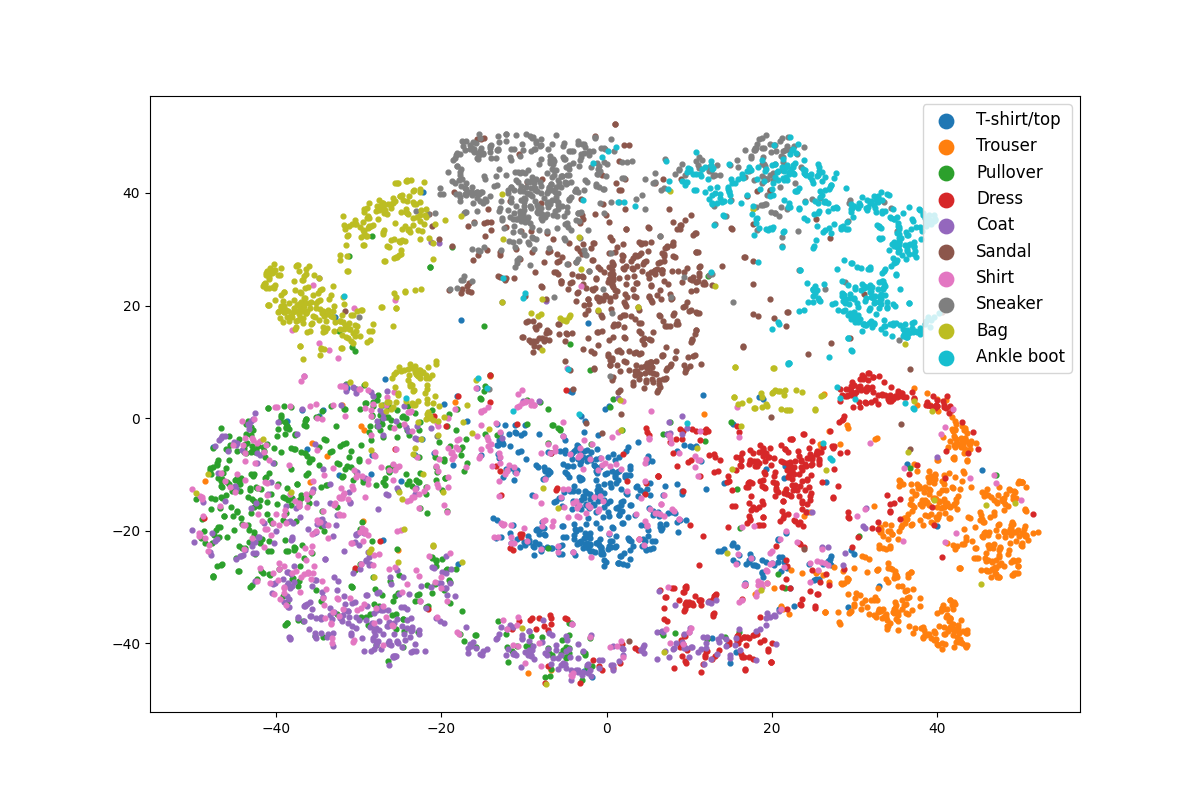
\includegraphics[width=1.0\textwidth]{../../out/activations_cnn/fmnist/t-sne/untrained/plot_l2_f0.png}
    \caption{Embeddings of activations in the second layer of an untrained neural network (t-SNE).}
\end{figure}

\begin{figure}
  \centering
    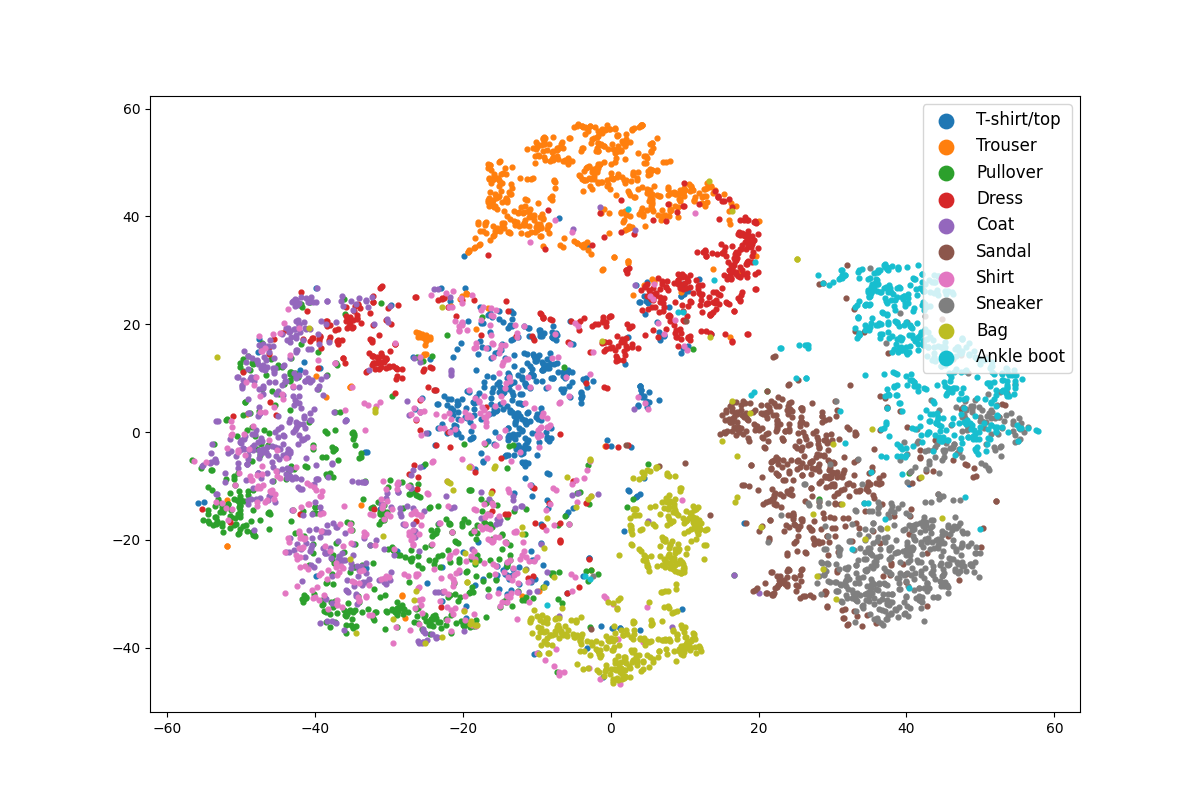
\includegraphics[width=1.0\textwidth]{../../out/activations_cnn/fmnist/t-sne/untrained/plot_l3.png}
    \caption{Embeddings of activations in the third layer of an untrained neural network (t-SNE).}
\end{figure}

The trend we observed in the case of MNIST dataset is present in this case
too. To make sure this is really the case, we compute values of metrics of
embedding quality and compare between the trained and the untrained network.
See Figures 38 to 43.

\begin{figure}
  \centering
    \resizebox{\textwidth}{!}{
        \begin{tabular}{llllll}
\toprule
{} &               ds &               dd &               cs &               cd &          acc\_knn \\
\midrule
filter 1 &  0.4190 / 0.4190 &  1.0646 / 1.0646 &  0.3117 / 0.3117 &  0.9527 / 0.9527 &  0.8328 / 0.8328 \\
\bottomrule
\end{tabular}

    }
  \caption{Values of metrics for embeddings acquired by t-SNE, original dataset.}
\end{figure}

\begin{figure}
  \centering
    \resizebox{\textwidth}{!}{
        \begin{tabular}{llllll}
\toprule
{} &               ds &               dd &               cs &               cd &          acc\_knn \\
\midrule
filter 1 &  0.9873 / 0.9848 &  1.0014 / 1.0017 &  0.7952 / 0.8904 &  0.3079 / 0.3053 &  0.1012 / 0.1084 \\
filter 2 &  0.4394 / 0.4577 &  1.0623 / 1.0603 &  0.3246 / 0.3335 &  0.9408 / 0.9308 &  0.8158 / 0.7830 \\
filter 3 &  0.9009 / 0.7268 &  1.0110 / 1.0304 &  0.7932 / 0.5390 &  0.4736 / 0.6707 &  0.2068 / 0.5576 \\
filter 4 &  0.3994 / 0.4192 &  1.0668 / 1.0646 &  0.2935 / 0.3081 &  0.9666 / 0.9551 &  0.8340 / 0.8134 \\
\bottomrule
\end{tabular}

    }
    \caption{Values of metrics for embeddings acquired by t-SNE, first layer.}
\end{figure}

\begin{figure}
  \centering
    \resizebox{\textwidth}{!}{
        \begin{tabular}{llllll}
\toprule
{} &               ds &               dd &               cs &               cd &          acc\_knn \\
\midrule
filter 1  &  0.5084 / 0.4670 &  1.0546 / 1.0593 &  0.3740 / 0.3380 &  0.8808 / 0.9186 &  0.7244 / 0.7672 \\
filter 2  &  0.5349 / 0.5292 &  1.0517 / 1.0523 &  0.3940 / 0.3880 &  0.8599 / 0.8772 &  0.7172 / 0.7110 \\
filter 3  &  0.5359 / 0.9431 &  1.0516 / 1.0063 &  0.3937 / 0.6762 &  0.8661 / 0.2595 &  0.7244 / 0.1690 \\
filter 4  &  0.5437 / 1.0017 &  1.0507 / 0.9998 &  0.4131 / 0.9410 &  0.8399 / 0.2029 &  0.7132 / 0.1016 \\
filter 5  &  0.4465 / 0.4365 &  1.0615 / 1.0626 &  0.3263 / 0.3177 &  0.9430 / 0.9420 &  0.7810 / 0.7814 \\
filter 6  &  0.5255 / 0.4312 &  1.0527 / 1.0632 &  0.3843 / 0.3120 &  0.8669 / 0.9430 &  0.7216 / 0.7812 \\
filter 7  &  0.5510 / 0.5872 &  1.0499 / 1.0459 &  0.4042 / 0.4306 &  0.8412 / 0.8213 &  0.6898 / 0.6542 \\
filter 8  &  0.5884 / 0.7899 &  1.0458 / 1.0234 &  0.4321 / 0.6837 &  0.8244 / 0.6114 &  0.7060 / 0.2494 \\
filter 9  &  0.5553 / 0.9931 &  1.0494 / 1.0008 &  0.4111 / 0.8814 &  0.8531 / 0.2709 &  0.6984 / 0.1060 \\
filter 10 &  0.5370 / 0.4733 &  1.0515 / 1.0585 &  0.3956 / 0.3455 &  0.8394 / 0.9102 &  0.7230 / 0.7714 \\
filter 11 &  0.5395 / 0.5819 &  1.0512 / 1.0465 &  0.3998 / 0.4373 &  0.8721 / 0.8305 &  0.7276 / 0.7010 \\
filter 12 &  0.6236 / 0.9583 &  1.0418 / 1.0046 &  0.4656 / 0.7442 &  0.7961 / 0.3636 &  0.6950 / 0.1350 \\
filter 13 &  0.6807 / 0.6936 &  1.0355 / 1.0341 &  0.5104 / 0.5441 &  0.6876 / 0.6840 &  0.6796 / 0.4448 \\
filter 14 &  0.5985 / 0.9720 &  1.0446 / 1.0031 &  0.4420 / 0.8357 &  0.8050 / 0.3537 &  0.6876 / 0.1310 \\
filter 15 &  0.4729 / 0.4339 &  1.0586 / 1.0629 &  0.3484 / 0.3145 &  0.9214 / 0.9404 &  0.7624 / 0.7824 \\
filter 16 &  0.6315 / 0.7519 &  1.0410 / 1.0276 &  0.4701 / 0.5599 &  0.7535 / 0.6404 &  0.7232 / 0.5594 \\
\bottomrule
\end{tabular}

    }
    \caption{Values of metrics for embeddings acquired by t-SNE, second layer.}
\end{figure}

\begin{figure}
  \centering
    \resizebox{\textwidth}{!}{
        \begin{tabular}{llllll}
\toprule
{} &               ds &               dd &               cs &               cd &          acc\_knn \\
\midrule
filter 1 &  0.3295 / 0.4415 &  1.0745 / 1.0621 &  0.2402 / 0.3221 &  1.0055 / 0.9358 &  0.8874 / 0.7856 \\
\bottomrule
\end{tabular}

    }
    \caption{Values of metrics for embeddings acquired by t-SNE, third layer.}
\end{figure}

\begin{figure}
  \centering
    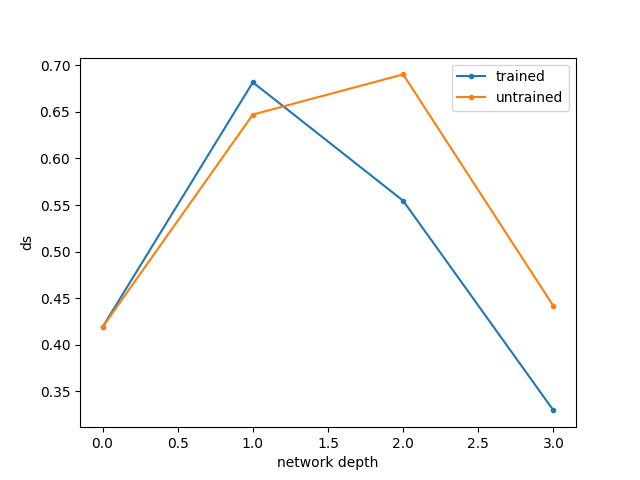
\includegraphics[width=0.75\textwidth]{../../out/activations_cnn/fmnist/t-sne/plot_metric_ds.png}
    \caption{Average value of the \(d_s\) metric (t-SNE).}
\end{figure}

\begin{figure}
  \centering
    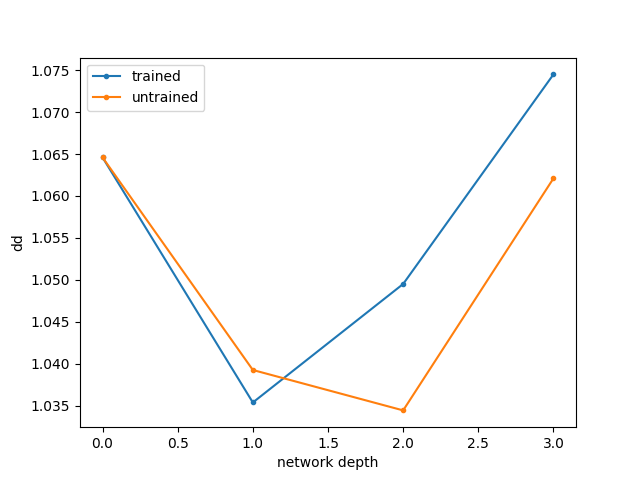
\includegraphics[width=0.75\textwidth]{../../out/activations_cnn/fmnist/t-sne/plot_metric_dd.png}
    \caption{Average value of the \(d_d\) metric (t-SNE).}
\end{figure}

We would like to look again a bit more closely at the outliers present
in the embeddings acquired from the third layer of the trained network.
We notice there is a big overlap between the Shirt and T-shirt/top
clusters. Figure 44 shows examples of these classes (as well as an
example that would be missclasified as Shirt even though it is a
T-shirt/top).

\begin{figure}
  \centering
  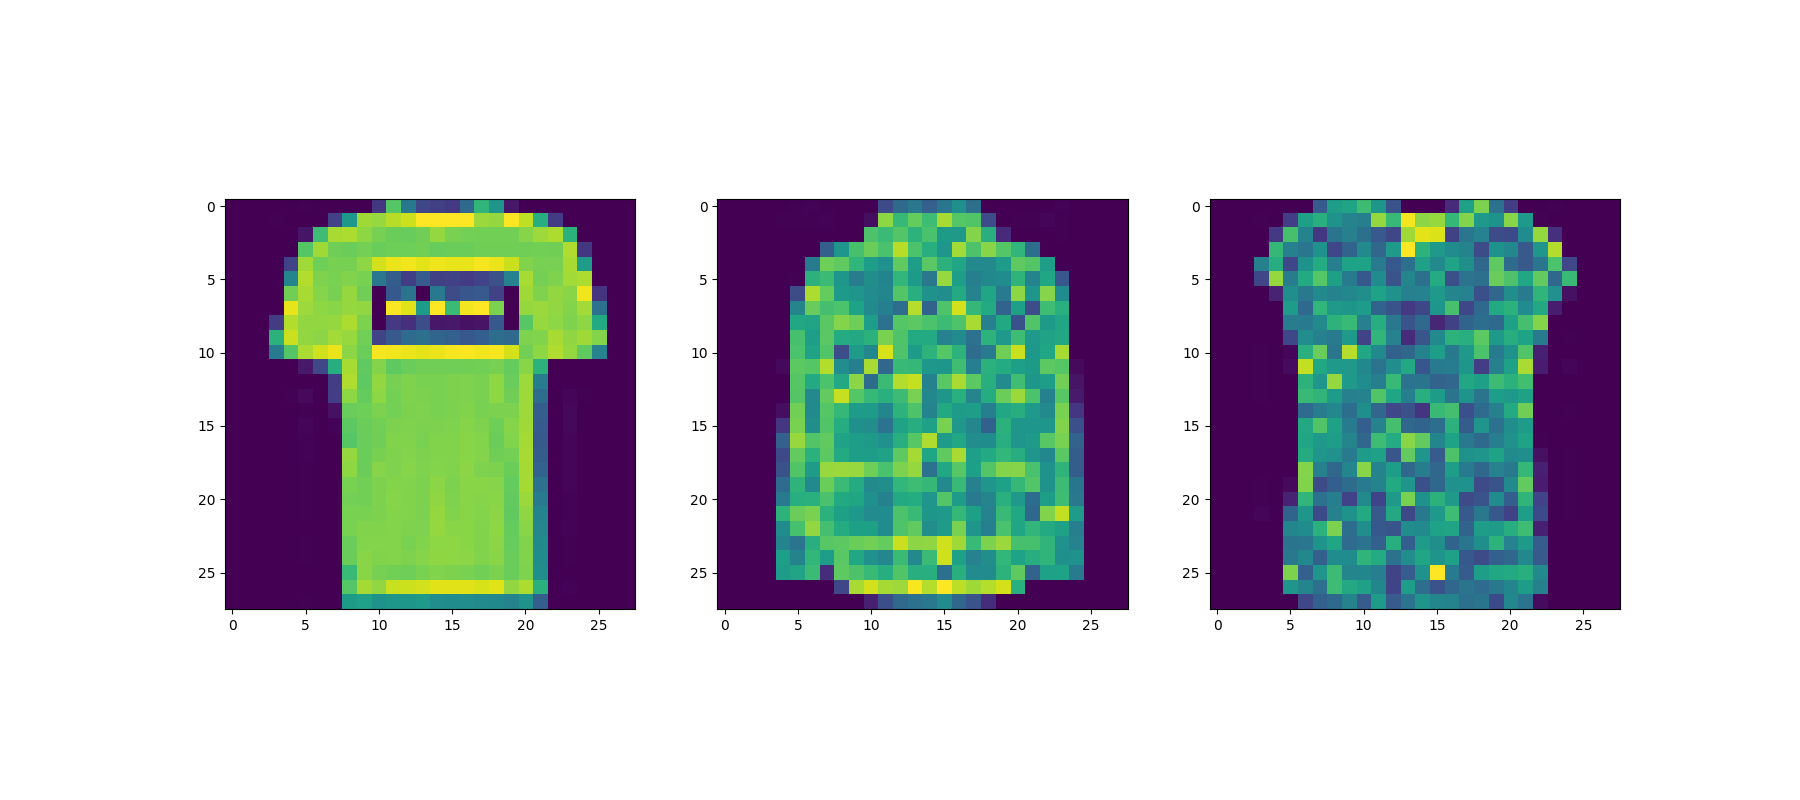
\includegraphics[width=0.75\textwidth]{../../out/activations_cnn/fmnist/t-sne/outliers/correct0_predicted6.png}
    \caption{From left: an example of T-shirt/top, an example of Shirt, the missclasified example.}
\end{figure}

We would also like to see what do the individual feature maps look like for
some example. We will use a T-shirt/top as such an example. Figures 45 to 47
contain these visualizations.

\begin{figure}
  \centering
  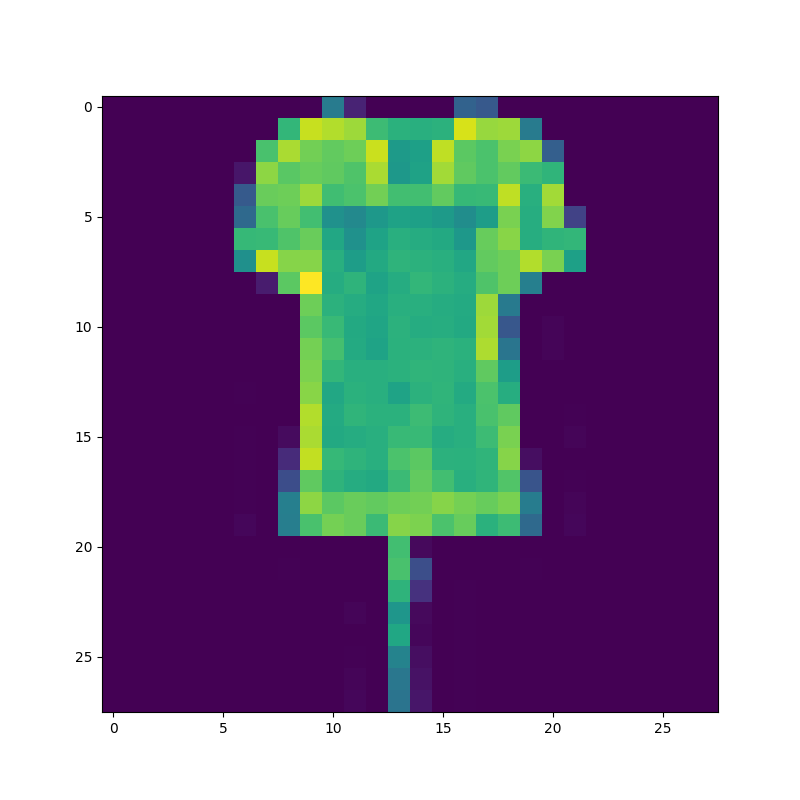
\includegraphics[width=0.75\textwidth]{../../out/activations_cnn/fmnist/t-sne/filter_outputs/class0_l0.png}
    \caption{An example of a T-shirt/top.}
\end{figure}

\begin{figure}
  \centering
  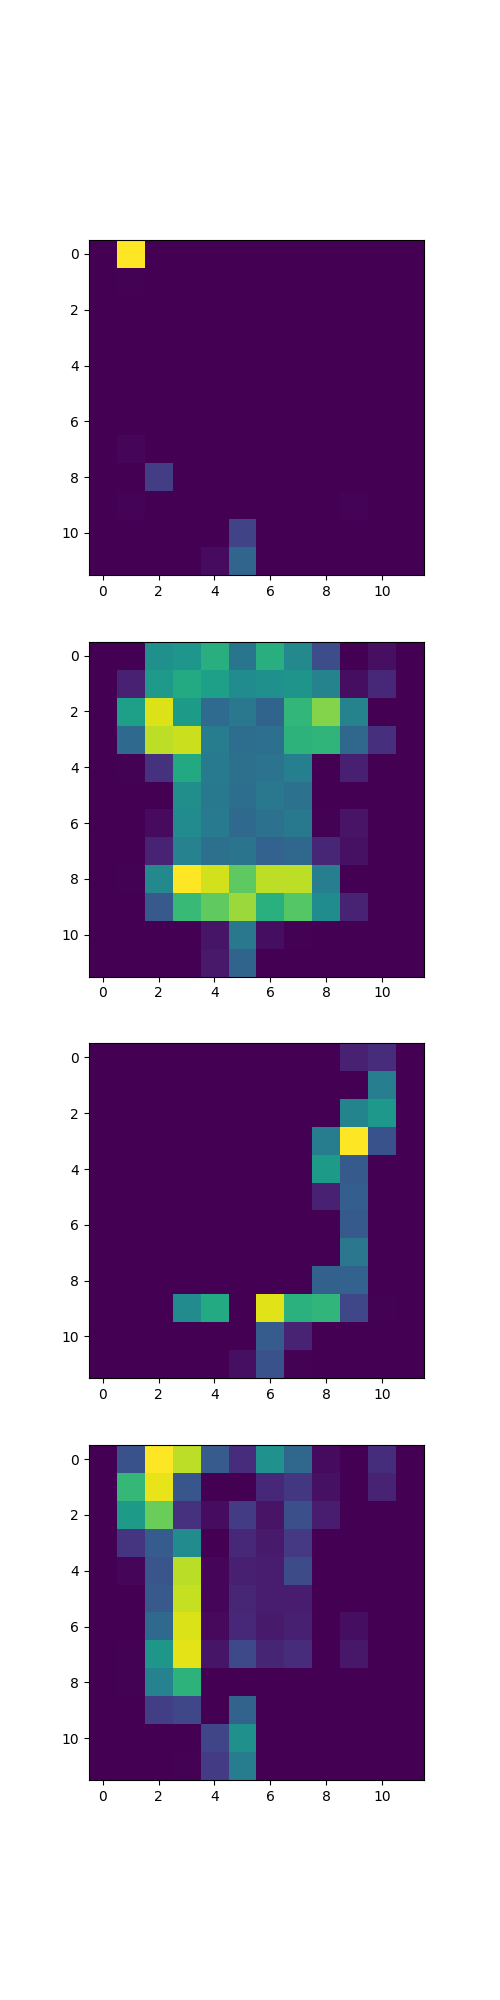
\includegraphics[width=0.25\textwidth]{../../out/activations_cnn/fmnist/t-sne/filter_outputs/class0_l1.png}
  \caption{Activations in the first layer of the network for the example.}
\end{figure}

\begin{figure}
  \centering
  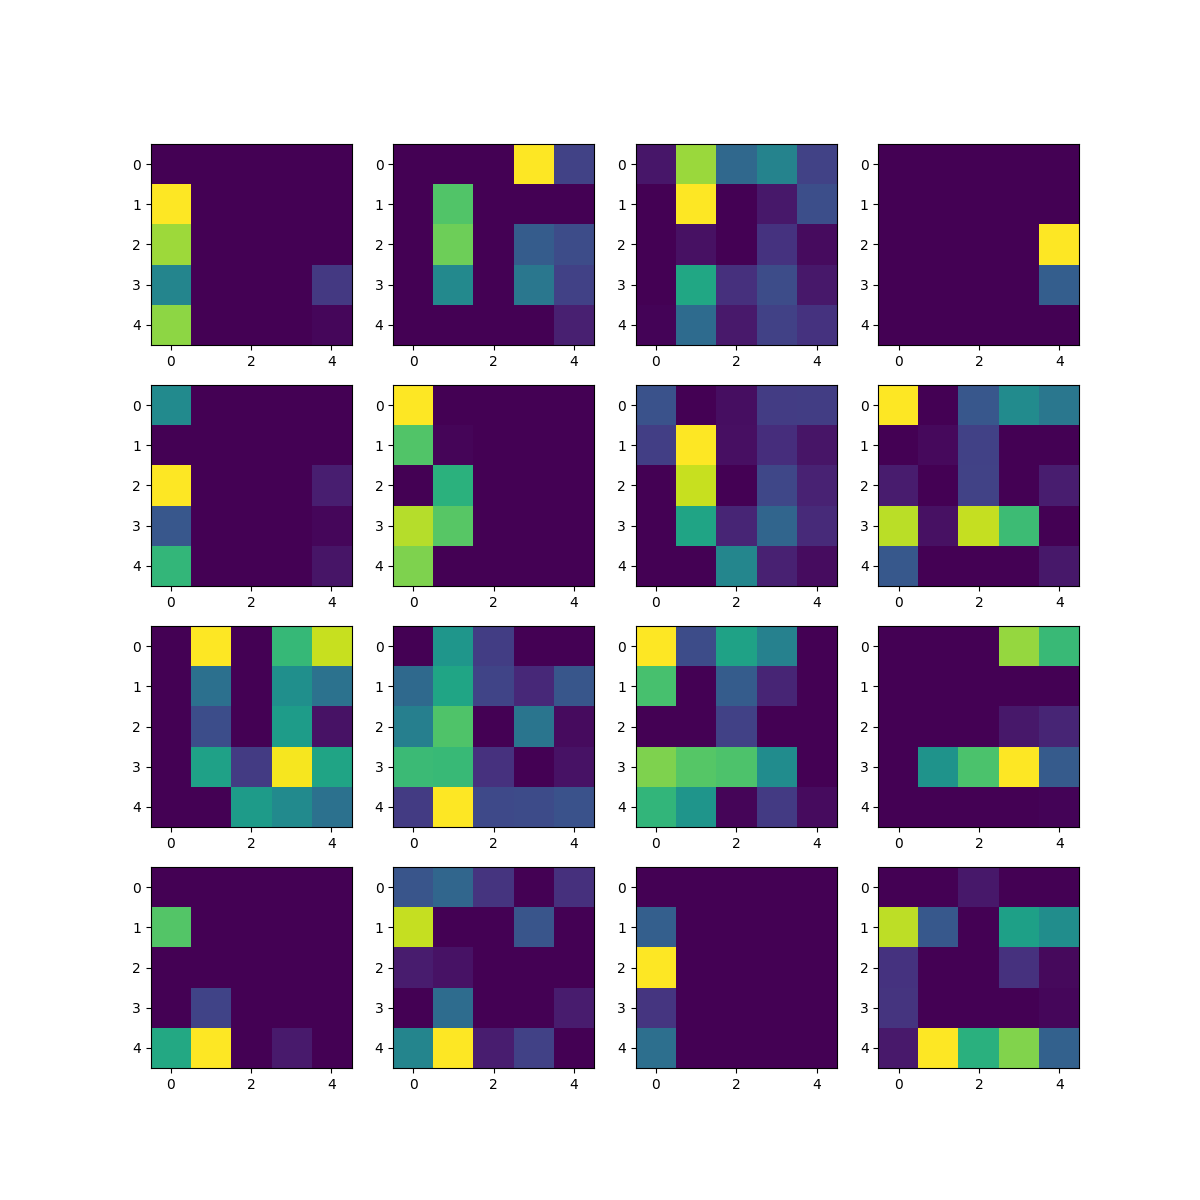
\includegraphics[width=0.75\textwidth]{../../out/activations_cnn/fmnist/t-sne/filter_outputs/class0_l2.png}
    \caption{Activations in the second layer of the network for the example.}
\end{figure}

Regarding the first layer, it is not clear what does the first filter
detect; the second filter seems to detect a transition from light pixels
to dark pixels in the top-bottom direction, and the third and fourth
filter seem to detect bottom right and upper left edge of a group
of light pixels, respectively. In the second layer, it is very hard to tell what meaning
each of the filters has.

Using UMAP to acquire embeddings, we get very similar results. Figures 48
to 54 show the computed embeddings.

\begin{figure}
  \centering
    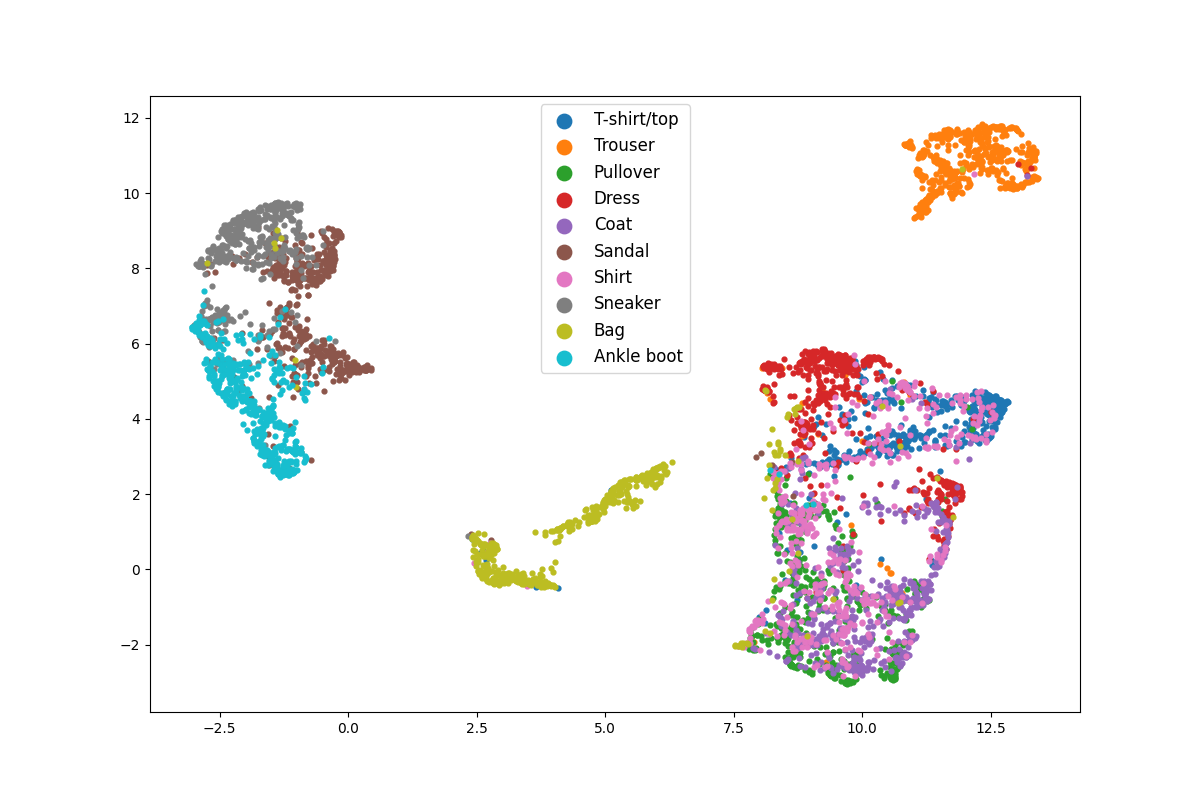
\includegraphics[width=1.0\textwidth]{../../out/activations_cnn/fmnist/umap/trained/plot_l0.png}
    \caption{Embeddings of the original dataset (UMAP).}
\end{figure}

\begin{figure}
  \centering
    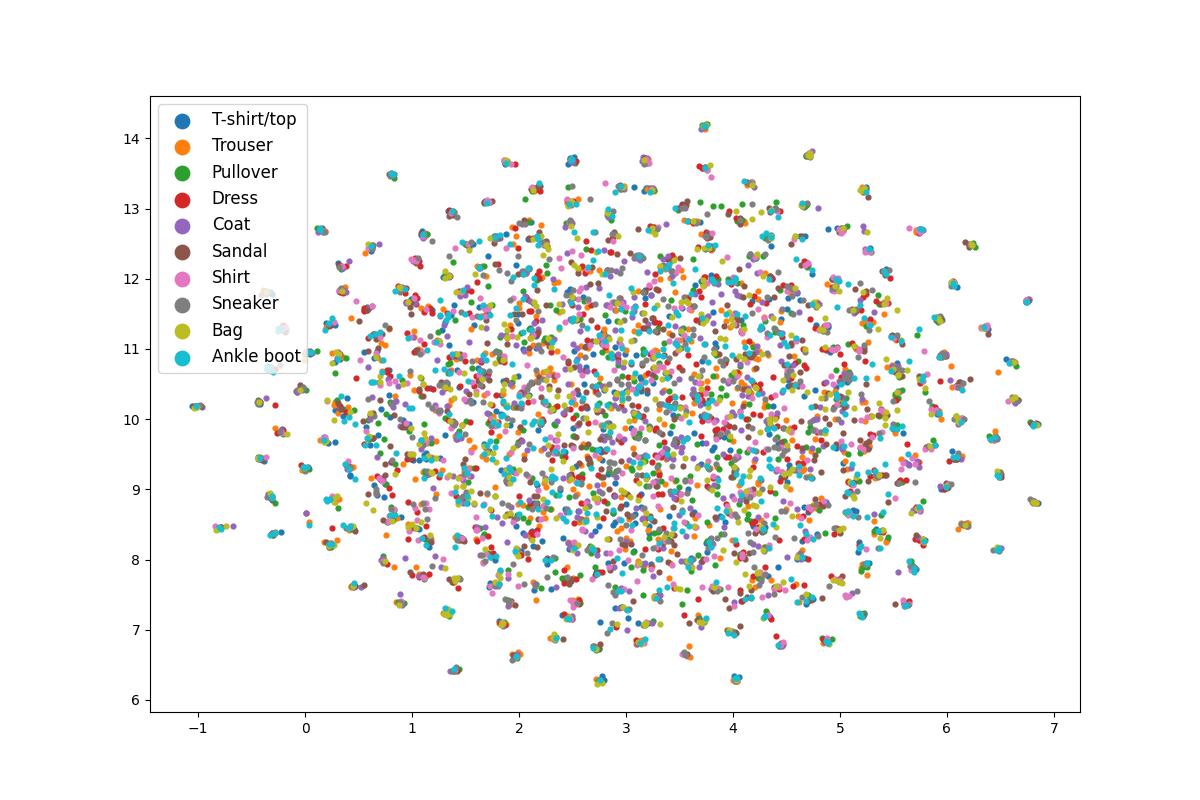
\includegraphics[width=1.0\textwidth]{../../out/activations_cnn/fmnist/umap/trained/plot_l1_f0.png}
    \caption{Embeddings of activations in the first layer of a neural network trained on FashionMNIST (UMAP).}
\end{figure}

\begin{figure}
  \centering
    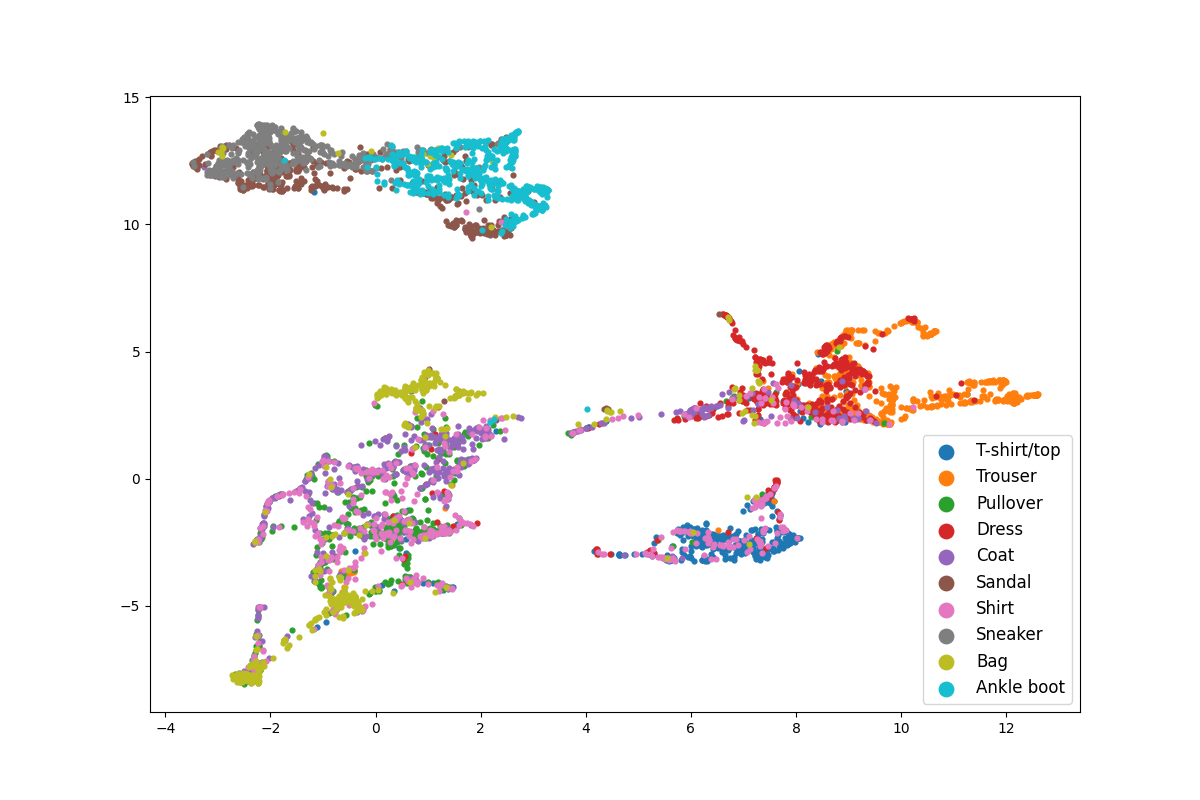
\includegraphics[width=1.0\textwidth]{../../out/activations_cnn/fmnist/umap/trained/plot_l2_f0.png}
    \caption{Embeddings of activations in the second layer of a neural network trained on FashionMNIST (UMAP).}
\end{figure}

\begin{figure}
  \centering
    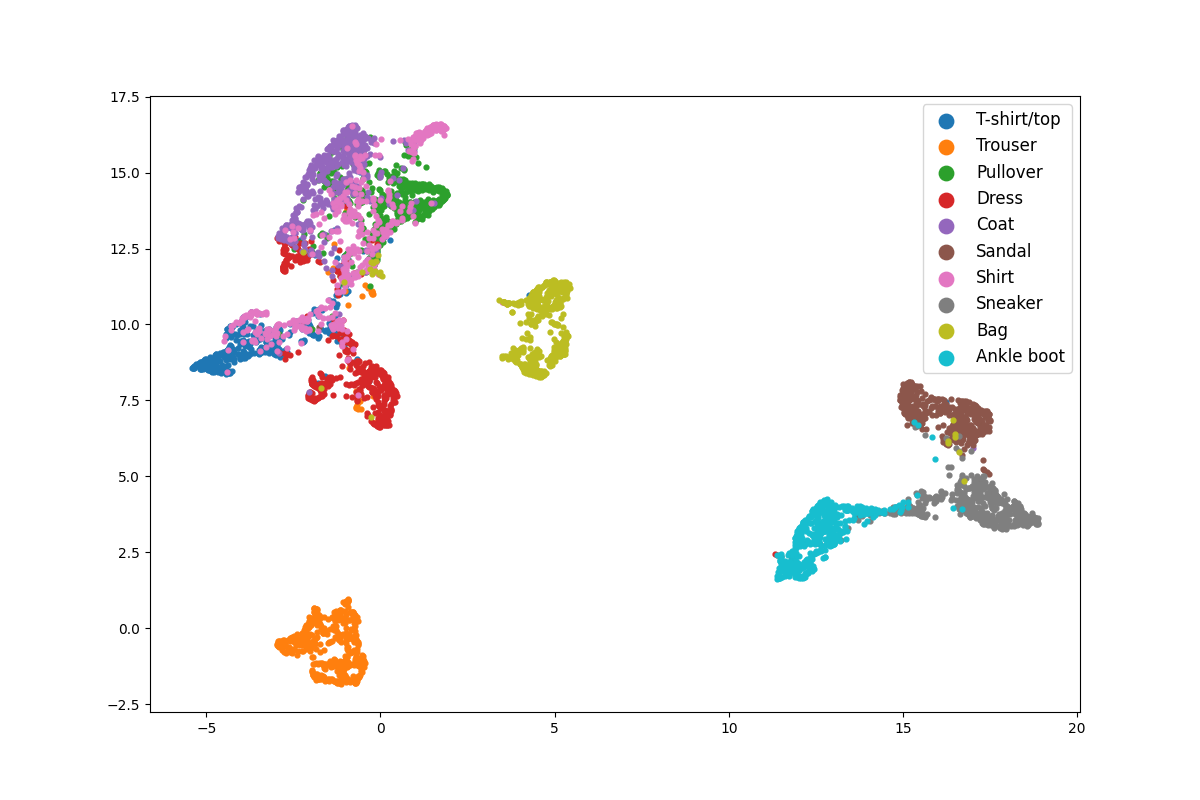
\includegraphics[width=1.0\textwidth]{../../out/activations_cnn/fmnist/umap/trained/plot_l3.png}
    \caption{Embeddings of activations in the third layer of a neural network trained on FashionMNIST (UMAP).}
\end{figure}

\begin{figure}
  \centering
    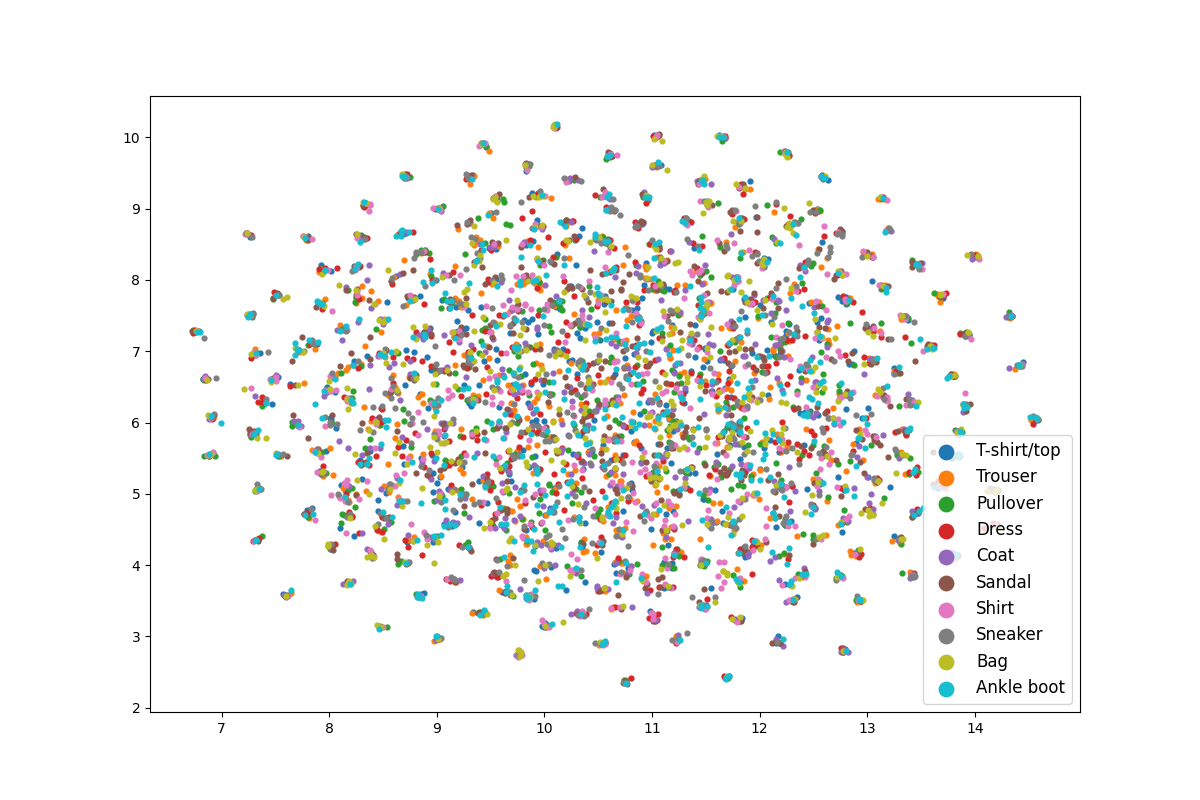
\includegraphics[width=1.0\textwidth]{../../out/activations_cnn/fmnist/umap/untrained/plot_l1_f0.png}
    \caption{Embeddings of activations in the first layer of an untrained neural network (UMAP).}
\end{figure}

\begin{figure}
  \centering
    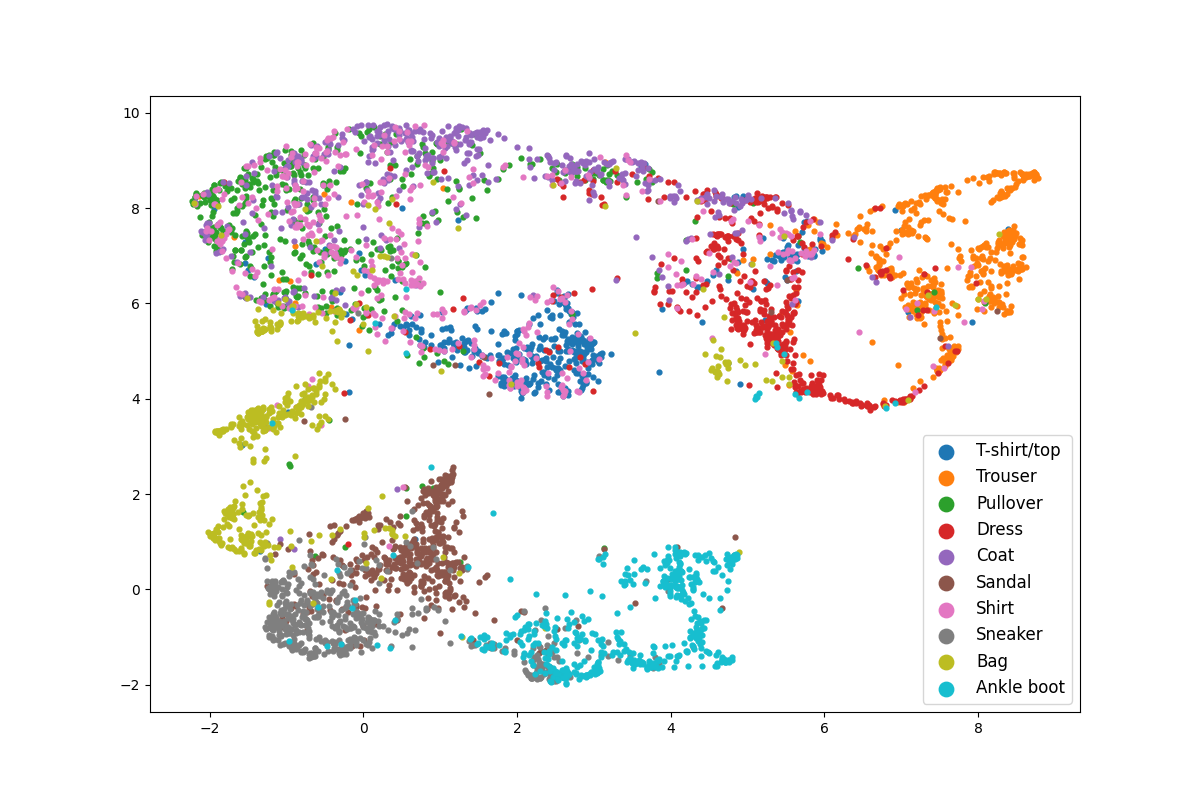
\includegraphics[width=1.0\textwidth]{../../out/activations_cnn/fmnist/umap/untrained/plot_l2_f0.png}
    \caption{Embeddings of activations in the second layer of an untrained neural network (UMAP).}
\end{figure}

\begin{figure}
  \centering
    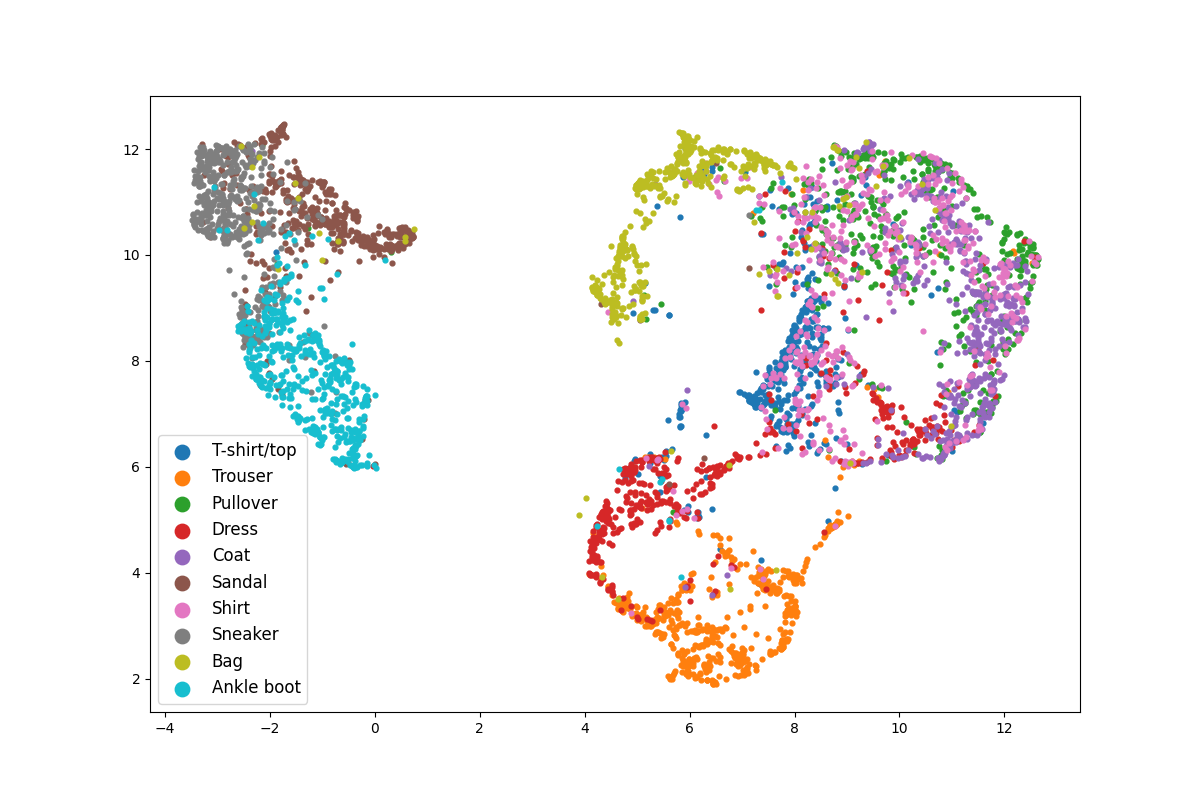
\includegraphics[width=1.0\textwidth]{../../out/activations_cnn/fmnist/umap/untrained/plot_l3.png}
    \caption{Embeddings of activations in the third layer of an untrained neural network (UMAP).}
\end{figure}

Again, we would like to confirm our observations by comparing values of
metrics over the computed embeddings. These can be seen in Figures 54 to
59.

\begin{figure}
  \centering
    \resizebox{\textwidth}{!}{
        \begin{tabular}{llllll}
\toprule
{} &               ds &               dd &               cs &               cd &          acc\_knn \\
\midrule
filter 1 &  0.2715 / 0.2744 &  1.0810 / 1.0807 &  0.1991 / 0.2017 &  1.0162 / 1.0154 &  0.8014 / 0.8078 \\
\bottomrule
\end{tabular}

    }
  \caption{Values of metrics for embeddings acquired by UMAP, original dataset.}
\end{figure}

\begin{figure}
  \centering
    \resizebox{\textwidth}{!}{
        \begin{tabular}{llllll}
\toprule
{} &               ds &               dd &               cs &               cd &          acc\_knn \\
\midrule
filter 1 &  1.0004 / 0.9999 &  1.0000 / 1.0000 &  0.7222 / 0.7213 &  0.0382 / 0.0504 &  0.2832 / 0.2762 \\
filter 2 &  0.2912 / 0.3710 &  1.0788 / 1.0699 &  0.2150 / 0.2711 &  1.0145 / 0.9738 &  0.7710 / 0.7546 \\
filter 3 &  0.9491 / 0.8821 &  1.0057 / 1.0131 &  0.6951 / 0.6522 &  0.2907 / 0.2972 &  0.3304 / 0.5526 \\
filter 4 &  0.2548 / 0.2902 &  1.0828 / 1.0789 &  0.1850 / 0.2116 &  1.0243 / 1.0118 &  0.8048 / 0.7932 \\
\bottomrule
\end{tabular}

    }
    \caption{Values of metrics for embeddings acquired by UMAP, first layer.}
\end{figure}

\begin{figure}
  \centering
    \resizebox{\textwidth}{!}{
        \begin{tabular}{llllll}
\toprule
{} &               ds &               dd &               cs &               cd &          acc\_knn \\
\midrule
filter 1  &  0.3698 / 0.4052 &  1.0701 / 1.0661 &  0.2717 / 0.2918 &  0.9546 / 0.9488 &  0.7144 / 0.7578 \\
filter 2  &  0.4812 / 0.4893 &  1.0577 / 1.0568 &  0.3524 / 0.3536 &  0.8889 / 0.8878 &  0.6960 / 0.6816 \\
filter 3  &  0.5024 / 0.9913 &  1.0553 / 1.0010 &  0.3714 / 0.7064 &  0.8888 / 0.1138 &  0.6978 / 0.2986 \\
filter 4  &  0.4162 / 1.0003 &  1.0649 / 1.0000 &  0.2992 / 0.7222 &  0.9375 / 0.0323 &  0.6936 / 0.2690 \\
filter 5  &  0.3514 / 0.3352 &  1.0721 / 1.0739 &  0.2563 / 0.2453 &  0.9913 / 0.9906 &  0.7658 / 0.7568 \\
filter 6  &  0.4769 / 0.3038 &  1.0581 / 1.0774 &  0.3494 / 0.2184 &  0.8998 / 1.0044 &  0.6982 / 0.7624 \\
filter 7  &  0.4869 / 0.5378 &  1.0570 / 1.0514 &  0.3545 / 0.3946 &  0.8674 / 0.8323 &  0.6756 / 0.6348 \\
filter 8  &  0.5598 / 0.8257 &  1.0489 / 1.0194 &  0.4134 / 0.6523 &  0.8421 / 0.5345 &  0.6744 / 0.3618 \\
filter 9  &  0.4940 / 0.9999 &  1.0562 / 1.0000 &  0.3639 / 0.7214 &  0.8914 / 0.0486 &  0.6700 / 0.2740 \\
filter 10 &  0.4605 / 0.3935 &  1.0600 / 1.0674 &  0.3337 / 0.2856 &  0.8934 / 0.9619 &  0.7012 / 0.7526 \\
filter 11 &  0.4727 / 0.5849 &  1.0586 / 1.0461 &  0.3525 / 0.4383 &  0.9189 / 0.8520 &  0.7118 / 0.6840 \\
filter 12 &  0.6188 / 0.9937 &  1.0424 / 1.0007 &  0.4627 / 0.7066 &  0.7985 / 0.1411 &  0.6734 / 0.2878 \\
filter 13 &  0.6530 / 0.6921 &  1.0386 / 1.0342 &  0.4908 / 0.5553 &  0.7295 / 0.6328 &  0.6484 / 0.5086 \\
filter 14 &  0.5699 / 0.9997 &  1.0478 / 1.0000 &  0.4244 / 0.7212 &  0.8216 / 0.0562 &  0.6620 / 0.2810 \\
filter 15 &  0.4351 / 0.3349 &  1.0628 / 1.0739 &  0.3201 / 0.2423 &  0.9299 / 0.9879 &  0.7588 / 0.7664 \\
filter 16 &  0.6159 / 0.7995 &  1.0427 / 1.0223 &  0.4639 / 0.6455 &  0.7569 / 0.6178 &  0.7032 / 0.5664 \\
\bottomrule
\end{tabular}

    }
    \caption{Values of metrics for embeddings acquired by UMAP, second layer.}
\end{figure}

\begin{figure}
  \centering
    \resizebox{\textwidth}{!}{
        \begin{tabular}{llllll}
\toprule
{} &               ds &               dd &               cs &               cd &          acc\_knn \\
\midrule
filter 1 &  0.1880 / 0.3332 &  1.0903 / 1.0741 &  0.1350 / 0.2420 &  1.0515 / 0.9892 &  0.8804 / 0.7640 \\
\bottomrule
\end{tabular}

    }
    \caption{Values of metrics for embeddings acquired by UMAP, third layer.}
\end{figure}

\begin{figure}
  \centering
    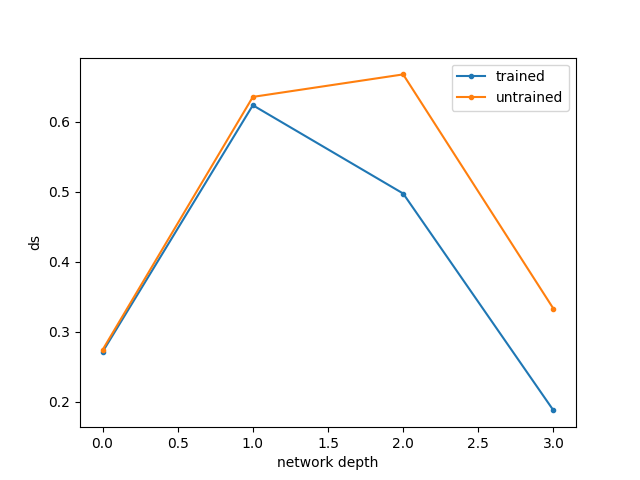
\includegraphics[width=0.75\textwidth]{../../out/activations_cnn/fmnist/umap/plot_metric_ds.png}
    \caption{Average value of the \(d_s\) metric (UMAP).}
\end{figure}

\begin{figure}
  \centering
    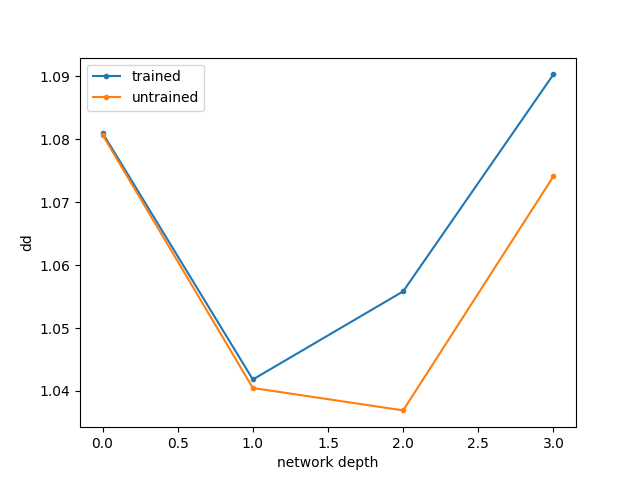
\includegraphics[width=0.75\textwidth]{../../out/activations_cnn/fmnist/umap/plot_metric_dd.png}
    \caption{Average value of the \(d_d\) metric (UMAP).}
\end{figure}

Again, the trend we are seeing both from the tables and from the plots is the
same one we noted when inspecting the embeddings visually.

\section{Conclusions}
In this work, we attempted to tackle the problem of data representation using
activations of a neural network. To find out whether these representations
are superior to their original counterparts, we compared them both visually
and using several metrics of embedding quality.

According to our results, the quality of embeddings acquired from a trained
network is in general better than the quality of embeddings acquired from
an untrained network irrespectively of depth of layer. Moreover, the quality
of embeddings acquired from the last layer of a network is generally better
than the embeddings computed from the original dataset in the case of
trained neural network, but not in the case of the untrained one.

Our results also suggest that by applying a convolutional filter a feature
map missing part of the information present in the original image is
obtained, and both in the case of trained and untrained network different
filters seem to extract different information from the original image.

\section{Future work}
We only used two very simple datasets, MNIST and FashionMNIST. Applying
our methods to more datasets is needed to ensure our results are not
specific to just these two datasets.

The metrics of embedding quality we used were rather arbitrary. A further
research into measures of embedding quality and their subsequent application
might make the obtained results more relevant.

The results were acquired by training the neural network once. To make
the results more reliable, several runs and a subsequent statistical
analysis would be a great step forward in terms of the quality of the
obtained results.

\end{document}



















